\documentclass[doubleside, titlepage]{article}
\usepackage{xcolor,listings}
\usepackage[utf8]{inputenc}
\usepackage[english]{babel}
\usepackage{textcomp}
\usepackage{graphicx}
\usepackage[papersize={210mm,297mm},top=2cm, bottom=2.25cm, left=1.8cm , right=1.8cm]{geometry}
\lstset{upquote=true}
\usepackage{amsmath}
\usepackage{tikz}
\usepackage{epigraph}
\usepackage{hyperref}
\hypersetup{
    linktoc=all
}
\usepackage{titlesec}
\usepackage{fancyhdr}
\pagestyle{fancy}
\usepackage{lastpage}

\renewcommand\headrulewidth{0.66pt}
\fancyhead[L]{\leftmark}
\fancyhead[R]{Spring 2016}

\renewcommand\footrulewidth{0.66pt}
\fancyfoot[L]{ ~\\ Group 3}
\fancyfoot[C]{ ~\\CS323 - Project delivrable \\ \textbf{Page \thepage/\pageref{LastPage}}}
\fancyfoot[R]{ ~\\ 
\includegraphics[scale=0.35]{epfl_logo}}

\fancypagestyle{firstpage}{%
    \fancyhf{}%
    \renewcommand\footrulewidth{0.66pt}
    \fancyfoot[L]{ ~\\ Group 3}
    \fancyfoot[C]{ ~\\CS323 - Project delivrable \\ \textbf{Page \thepage/\pageref{LastPage}}}
    \fancyfoot[R]{ ~\\ 
\includegraphics[scale=0.35]{epfl_logo}}
    \renewcommand{\headrulewidth}{0mm}%
}

\renewcommand\epigraphflush{center}
\renewcommand\epigraphsize{\normalsize}
\setlength\epigraphwidth{0.5\textwidth}
\setlength\epigraphrule{0.5pt}

\renewcommand{\textflush}{flushright} \renewcommand{\sourceflush}{flushright}

\let\originalepigraph\epigraph
\renewcommand\epigraph[2]{\originalepigraph{#1}{\textsc{#2}}}

\definecolor{titlepagecolor}{cmyk}{0,.9,0.7,0}

\DeclareFixedFont{\titlefont}{T1}{ppl}{b}{}{0.5in}

\makeatletter
\def\printauthor{%
    {\large \@author}}
\makeatother
\author{%
	~\\	~\\
    Jeremy Hottinger \\
    259573 \\
    \href{mailto:jeremy.hottinger@epfl.ch}{\texttt{jeremy.hottinger@epfl.ch}}\vspace{20pt} \\
    Aurelien Soccard \\
    235746 \\
    \href{mailto:aurelien.soccard@epfl.ch}{\texttt{aurelien.soccard@epfl.ch}}\vspace{20pt} \\
    Teo Stocco \\
    235744 \\
    \href{mailto:teo.stocco@epfl.ch}{\texttt{teo.stocco@epfl.ch}}\vspace{20pt} \\
    }

% The following code is borrowed from: http://tex.stackexchange.com/a/86310/10898

\newcommand\titlepagedecoration{%
\begin{tikzpicture}[remember picture,overlay,shorten >= -10pt]

\coordinate (aux1) at ([yshift=-15pt]current page.north east);
\coordinate (aux2) at ([yshift=-410pt]current page.north east);
\coordinate (aux3) at ([xshift=-4.5cm]current page.north east);
\coordinate (aux4) at ([yshift=-150pt]current page.north east);

\begin{scope}[titlepagecolor!40,line width=12pt,rounded corners=12pt]
\draw
  (aux1) -- coordinate (a)
  ++(225:5) --
  ++(-45:5.1) coordinate (b);
\draw[shorten <= -10pt]
  (aux3) --
  (a) --
  (aux1);
\draw[opacity=0.6,titlepagecolor,shorten <= -10pt]
  (b) --
  ++(225:2.2) --
  ++(-45:2.2);
\end{scope}
\draw[titlepagecolor,line width=8pt,rounded corners=8pt,shorten <= -10pt]
  (aux4) --
  ++(225:0.8) --
  ++(-45:0.8);
\begin{scope}[titlepagecolor!70,line width=6pt,rounded corners=8pt]
\draw[shorten <= -10pt]
  (aux2) --
  ++(225:3) coordinate[pos=0.45] (c) --
  ++(-45:3.1);
\draw
  (aux2) --
  (c) --
  ++(135:2.5) --
  ++(45:2.5) --
  ++(-45:2.5) coordinate[pos=0.3] (d);
\draw
  (d) -- +(45:1);
\end{scope}
\end{tikzpicture}%
}

\begin{document}
\begin{titlepage}
\thispagestyle{firstpage}
\vspace*{3cm}
\titlefont CS-323 : Project delivrable\par
\vspace*{0.5cm}
\epigraph{This is our deliverable for the \textit{Bookshelf} project of the introduction to database course (spring 2016 - Pr. Anastasia Ailamaki), which sums up our work.~\\ It also contains some justifications.}%
{\textit{May 2016} - \textsc{Team 3}}
\null\vfill
\vspace*{5cm}
\noindent
\hfill
\begin{minipage}{0.5\linewidth}
    \begin{flushright}
        \printauthor
    \end{flushright}
\end{minipage}
%
\begin{minipage}{0.02\linewidth}
    \rule{1pt}{175pt}
\end{minipage}
\titlepagedecoration
\end{titlepage}

\setcounter{tocdepth}{3}
\vspace{-1cm}
\tableofcontents

\newpage

\part{Delivrable 1}

\section{Justifications}

We started to take a look at the given data and tried to understand how tables where connected at a first glance by drawing a really simplified diagram. Once this was done, we started to look at more deeply to the data : how are they stored? May they be empty? Are they all relevant? Our major decision was not to drop any table, but only add and remove some fields to entities.
~\\~\\
First, for everything that is related to publications, we quickly figured out how things were working. Therefore, we quickly decided to drop some of the unused id (such as its publication author or its publication content). As a primary key, we made the choice to inflate it using constraints. Furthermore, we also decided to separate the price into two fields, one for the amount and one for the currency, this solution being much more efficient while looking for some price range for instance.
~\\~\\
Even though both publications and titles have each one a related type field we did not find it relevant to split them into different tables and/or explicit a IS-A relationship because of the way the datas are gathered.
~\\~\\
Another part of the work was to analyse how tables were connected to remove potential redundancy. For instance, an award has a category but also a type, and a category has a type. These two types being always the same, we needed to drop out some content, what we've done by removing the type entry in a award. We also realise that, for instance in the author table, among the 80'000 birth places, only 10\% were unique so we have started thinking about changing this attribute into a placeID and create a places table. There were some advantages (no redundancy, less space consumed) but some drawbacks (2 queries instead of one for each author) that finally made us stay with the given configuration (however, if another would be using a place, we will have done that).
~\\~\\
Furthermore, to write properly the creation of the table, we needed to know exactly what entry may be null, and which ones could not. This was done by inspecting carefully the data and reading correctly the instructions. Then, the dilemma was for notes and web pages tables. Indeed, for note, we only have two entries : the ID and the raw note, whereas for a website, there are an ID, an URL but also some other IDs to relate it to other entities : among these 7 IDs, only one   The type of each entry is explained in the following paragraph. Our final has been not the change the structure of these two tables since there is no WebpageID entry in tables as there is for note, but whether a web page is directly connected to the ID of its corresponding entity. Therefore, it implies to add an entry into these 7 tables, and we decided not to do this for practical reasons. Besides, we also thought about simply adding a simply URL entry into the note table, but this solution was also not satisfactory since before insert we would need to do a map from web page to note (not that hard) but since primary keys are only unique in one table, an author and a publication may have the same ID and this would imply much more work to know which website belongs to who.
~\\~\\
As publications and titles both have a type we used an enum as a compromise between having a raw string field and creating normalisation for it. This avoids the redundancy and increase data consistency. Note that it would not be an option if the dataset usage would include adding new types (normalising is better in this case).
~\\~\\
Last but not least, some intensive parsing has also been performed to know exactly how many characters were required for instance for each field, since we have encountered some difficulties with Cyrillic. We quickly realised that we should definitely parse these values before inserting them, it presents the advantages of being less memory consuming (6 characters become 1) and also the process of conversion is only done one time.
\addtocounter{page}{1}

\section{ER model}

This entity-relation model only contains fields which are either directly use for relation or as primary key (underline then). For a more complete view of the table, refers to the next section. Fields are coloured in blue, direct relationships in yellow, relationships through a table in red.
~\\
\textbf{Note :} If you find this diagram too small, a larger version is available online at the following address :
$$
\text{\href{https://documents.epfl.ch/users/s/so/soccard/private/DBMS}{\texttt{https://documents.epfl.ch/users/s/so/soccard/private/DBMS}}}
$$
\begin{flushright}
(access restricted to the db2016 group as defined in the EPFL AD directory).
\end{flushright}

\newpage

\begin{center}
    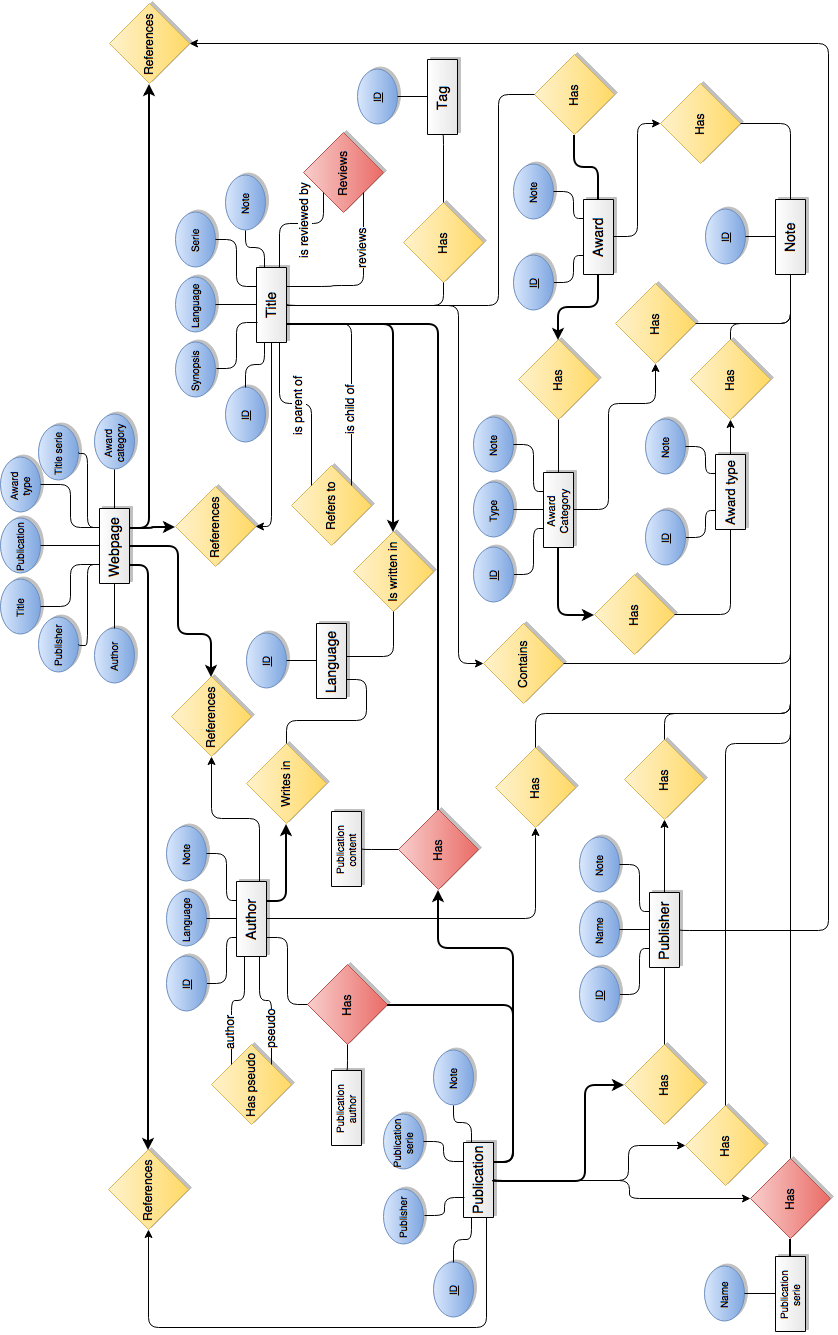
\includegraphics[scale = 0.5]{DBMS_ER_OLD}
\end{center}

\section{SQL schema}

\subsection{Entities}

\begin{lstlisting}[language=SQL,showspaces=false,basicstyle=\ttfamily,numberstyle=\tiny,commentstyle=\color{gray}
        ]
CREATE TYPE PUBLICATION_TYPE AS ENUM ('ANTHOLOGY', 'COLLECTION', 'MAGAZINE',
	'NONFICTION', 'NOVEL', 'OMNIBUS', 'FANZINE', 'CHAPBOOK');
\end{lstlisting}

\begin{lstlisting}[language=SQL,showspaces=false,basicstyle=\ttfamily,numberstyle=\tiny,commentstyle=\color{gray}
        ]
CREATE TYPE TITLE_TYPE AS ENUM ('ANTHOLOGY', 'BACKCOVERART', 'COLLECTION',
	'COVERART', 'INTERIORART', 'EDITOR', 'ESSAY', 'INTERVIEW', 'NOVEL',
	'NONFICTION', 'OMNIBUS', 'POEM', 'REVIEW', 'SERIAL', 'SHORTFICTION',
	'CHAPBOOK');
\end{lstlisting}

\begin{lstlisting}[language=SQL,showspaces=false,basicstyle=\ttfamily,numberstyle=\tiny,commentstyle=\color{gray}
        ]
CREATE TABLE authors
(
  id          INT PRIMARY KEY NOT NULL,
  name        VARCHAR(256)    NOT NULL,
  legal_name  VARCHAR(256),
  last_name   VARCHAR(256),
  pseudonym   INT, -- fk
  birth_place VARCHAR(256),
  birth_date  DATE,
  death_date  DATE,
  email       VARCHAR(256),
  image       VARCHAR(256),
  language_id INT, -- fk
  note_id     INT -- fk
)
\end{lstlisting}

\begin{lstlisting}[language=SQL,showspaces=false,basicstyle=\ttfamily,numberstyle=\tiny,commentstyle=\color{gray}
        ]
CREATE TABLE publications
(
  id             INT PRIMARY KEY 	NOT NULL,
  title          VARCHAR(256)    	NOT NULL,
  date_pub       DATE            	NOT NULL,
  publisher_id   INT             	NOT NULL, -- fk
  pages          INT,
  preface        INT,
  packaging_type VARCHAR(16)   		NOT NULL,
  type           PUBLICATON_TYPE    NOT NULL,
  isbn           BIGINT,
  cover          VARCHAR(256),
  price          FLOAT,
  currency       VARCHAR(8),
  pub_series_id  INT, -- fk
  pub_series_num INT,
  note_id        INT -- fk
)
\end{lstlisting}

\newpage

\begin{lstlisting}[language=SQL,showspaces=false,basicstyle=\ttfamily,numberstyle=\tiny,commentstyle=\color{gray}
        ]
CREATE TABLE titles
(
  id           INT PRIMARY KEY NOT NULL,
  title        VARCHAR(256)    NOT NULL,
  translator   VARCHAR(256),
  synopsis     INT, -- fk
  note_id      INT, -- fk
  series_id    INT, -- fk
  series_num   INT,
  story_length VARCHAR(256),
  type         TITLE_TYPE,
  parent       INT             NOT NULL DEFAULT 0, -- fk
  language_id  INT, -- fk
  graphic      BOOLEAN         NOT NULL
)
\end{lstlisting}

\begin{lstlisting}[language=SQL,showspaces=false,basicstyle=\ttfamily,numberstyle=\tiny,commentstyle=\color{gray}
        ]
CREATE TABLE languages
(
  id     INT PRIMARY KEY NOT NULL,
  name   VARCHAR(256)    NOT NULL,
  code   CHAR(3)         NOT NULL UNIQUE,
  script BOOLEAN
)
\end{lstlisting}

\begin{lstlisting}[language=SQL,showspaces=false,basicstyle=\ttfamily,numberstyle=\tiny,commentstyle=\color{gray}
        ]
CREATE TABLE notes
(
  id   INT PRIMARY KEY NOT NULL,
  note TEXT            NOT NULL
)
\end{lstlisting}

\begin{lstlisting}[language=SQL,showspaces=false,basicstyle=\ttfamily,numberstyle=\tiny,commentstyle=\color{gray}
        ]
CREATE TABLE webpages
(
  id                     INT PRIMARY KEY NOT NULL,
  author_id              INT, -- fk
  publisher_id           INT, -- fk
  title_id               INT, -- fk
  url                    VARCHAR(256)    NOT NULL UNIQUE,
  publications_series_id INT, -- fk
  award_type_id          INT, -- fk
  title_series_id        INT, -- fk
  award_category_id      INT -- fk
)
\end{lstlisting}

\begin{lstlisting}[language=SQL,showspaces=false,basicstyle=\ttfamily,numberstyle=\tiny,commentstyle=\color{gray}
        ]
CREATE TABLE tags
(
  id   INT PRIMARY KEY NOT NULL,
  name VARCHAR(256)    NOT NULL
)
\end{lstlisting}

\begin{lstlisting}[language=SQL,showspaces=false,basicstyle=\ttfamily,numberstyle=\tiny,commentstyle=\color{gray}
        ]
CREATE TABLE titles_series
(
  id      INT PRIMARY KEY NOT NULL,
  title   VARCHAR(256)    NOT NULL,
  parent  INT DEFAULT 0, -- fk
  note_id INT -- fk
)
\end{lstlisting}

\newpage

\begin{lstlisting}[language=SQL,showspaces=false,basicstyle=\ttfamily,numberstyle=\tiny,commentstyle=\color{gray}
        ]
CREATE TABLE awards
(
  id          INT PRIMARY KEY NOT NULL,
  title       VARCHAR(256)    NOT NULL,
  date        DATE            NOT NULL,
  category_id INT             NOT NULL, -- fk
  note_id     INT -- fk
)
\end{lstlisting}

\begin{lstlisting}[language=SQL,showspaces=false,basicstyle=\ttfamily,numberstyle=\tiny,commentstyle=\color{gray}
        ]
CREATE TABLE awards_categories
(
  id      INT PRIMARY KEY NOT NULL,
  name    VARCHAR(256)    NOT NULL,
  type_id INT             NOT NULL, -- fk
  ordr    INT,
  note_id INT -- fk
)
\end{lstlisting}

\begin{lstlisting}[language=SQL,showspaces=false,basicstyle=\ttfamily,numberstyle=\tiny,commentstyle=\color{gray}
        ]
CREATE TABLE awards_types
(
  id          INT PRIMARY KEY NOT NULL,
  code        CHAR(2) UNIQUE,
  name        VARCHAR(256)    NOT NULL,
  note_id     INT, -- fk
  awarded_by  VARCHAR(256)    NOT NULL,
  awarded_for VARCHAR(256)    NOT NULL,
  short_name  VARCHAR(256)    NOT NULL UNIQUE,
  poll        BOOLEAN         NOT NULL,
  non_genre   BOOLEAN         NOT NULL
)
\end{lstlisting}

\begin{lstlisting}[language=SQL,showspaces=false,basicstyle=\ttfamily,numberstyle=\tiny,commentstyle=\color{gray}
        ]
CREATE TABLE publishers
(
  id      INT PRIMARY KEY NOT NULL,
  name    VARCHAR(512)    NOT NULL,
  note_id INT -- fk
)
\end{lstlisting}

\begin{lstlisting}[language=SQL,showspaces=false,basicstyle=\ttfamily,numberstyle=\tiny,commentstyle=\color{gray}
        ]
CREATE TABLE publications_series
(
  id      INT PRIMARY KEY NOT NULL,
  name    VARCHAR(512)    NOT NULL,
  note_id INT -- fk
)
\end{lstlisting}

\subsection{Relations}

\begin{lstlisting}[language=SQL,showspaces=false,basicstyle=\ttfamily,numberstyle=\tiny,commentstyle=\color{gray}
        ]
CREATE TABLE publications_authors
(
  publication_id INT NOT NULL, -- fk
  author_id      INT NOT NULL, -- fk
  CONSTRAINT pk_publications_authors PRIMARY KEY (publication_id, author_id)
)
\end{lstlisting}

\begin{lstlisting}[language=SQL,showspaces=false,basicstyle=\ttfamily,numberstyle=\tiny,commentstyle=\color{gray}
        ]
CREATE TABLE titles_awards
(
  title_id INT NOT NULL, -- fk
  award_id INT NOT NULL, -- fk
  CONSTRAINT pk_titles_awards PRIMARY KEY (title_id, award_id)
)
\end{lstlisting}

\begin{lstlisting}[language=SQL,showspaces=false,basicstyle=\ttfamily,numberstyle=\tiny,commentstyle=\color{gray}
        ]
CREATE TABLE titles_tags
(
  title_id INT NOT NULL, -- fk
  tag_id   INT NOT NULL, -- fk
  CONSTRAINT pk_titles_tags PRIMARY KEY (title_id, tag_id)
)
\end{lstlisting}

\begin{lstlisting}[language=SQL,showspaces=false,basicstyle=\ttfamily,numberstyle=\tiny,commentstyle=\color{gray}
        ]
CREATE TABLE reviews
(
  title_id  INT NOT NULL, -- fk
  review_id INT NOT NULL, -- fk
  CONSTRAINT pk_reviews PRIMARY KEY (title_id, review_id)
)
\end{lstlisting}

\begin{lstlisting}[language=SQL,showspaces=false,basicstyle=\ttfamily,numberstyle=\tiny,commentstyle=\color{gray}
        ]
CREATE TABLE publications_contents
(
  title_id       INT NOT NULL, -- fk
  publication_id INT NOT NULL, -- fk
  CONSTRAINT pk_publications_contents PRIMARY KEY (title_id, publication_id)
)
\end{lstlisting}


\subsection{Foreign keys}

\subsubsection{Authors}
\begin{tabular}{ ll }
\begin{minipage}{3in}
\begin{lstlisting}[language=SQL,showspaces=false,basicstyle=\ttfamily,numberstyle=\tiny,commentstyle=\color{gray}
        ]
ALTER TABLE authors
ADD FOREIGN KEY (language_id)
REFERENCES languages (id)
ON DELETE SET NULL;
\end{lstlisting}
\end{minipage}
&
\begin{minipage}{3in}
\begin{lstlisting}[language=SQL,showspaces=false,basicstyle=\ttfamily,numberstyle=\tiny,commentstyle=\color{gray}
        ]
ALTER TABLE authors
ADD FOREIGN KEY (pseudonym)
REFERENCES authors (id)
ON DELETE CASCADE;
\end{lstlisting}
\end{minipage}
\\
\begin{minipage}{3in}
\begin{lstlisting}[language=SQL,showspaces=false,basicstyle=\ttfamily,numberstyle=\tiny,commentstyle=\color{gray}
        ]
ALTER TABLE authors
ADD FOREIGN KEY (note_id)
REFERENCES notes (id)
ON DELETE SET NULL;
\end{lstlisting}

\end{minipage}
\end{tabular}

\subsubsection{Publication authors}
\begin{tabular}{ ll }
\begin{minipage}{3in}
\begin{lstlisting}[language=SQL,showspaces=false,basicstyle=\ttfamily,numberstyle=\tiny,commentstyle=\color{gray}
        ]
ALTER TABLE publications_authors
ADD FOREIGN KEY (publication_id)
REFERENCES publications (id)
ON DELETE CASCADE;
\end{lstlisting}
\end{minipage}
&
\begin{minipage}{3in}
\begin{lstlisting}[language=SQL,showspaces=false,basicstyle=\ttfamily,numberstyle=\tiny,commentstyle=\color{gray}
        ]
ALTER TABLE publications_authors
ADD FOREIGN KEY (author_id)
REFERENCES authors (id)
ON DELETE CASCADE;
\end{lstlisting}
\end{minipage}
\end{tabular}

\subsubsection{Publications}
\begin{tabular}{ ll }
\begin{minipage}{3in}
\begin{lstlisting}[language=SQL,showspaces=false,basicstyle=\ttfamily,numberstyle=\tiny,commentstyle=\color{gray}
        ]
ALTER TABLE publications
ADD FOREIGN KEY (publisher_id)
REFERENCES publishers (id)
ON DELETE SET NULL;
\end{lstlisting}
\end{minipage}
&
\begin{minipage}{3in}
\begin{lstlisting}[language=SQL,showspaces=false,basicstyle=\ttfamily,numberstyle=\tiny,commentstyle=\color{gray}
        ]
ALTER TABLE publications
ADD FOREIGN KEY (pub_series_id)
REFERENCES publications_series (id)
ON DELETE SET NULL;
\end{lstlisting}
\end{minipage}
\\
\begin{minipage}{3in}
\begin{lstlisting}[language=SQL,showspaces=false,basicstyle=\ttfamily,numberstyle=\tiny,commentstyle=\color{gray}
        ]
ALTER TABLE publications
ADD FOREIGN KEY (note_id)
REFERENCES notes (id)
ON DELETE SET NULL;
\end{lstlisting}
\end{minipage}
\end{tabular}

\subsubsection{Publication contents}
\begin{tabular}{ ll }
\begin{minipage}{3in}
\begin{lstlisting}[language=SQL,showspaces=false,basicstyle=\ttfamily,numberstyle=\tiny,commentstyle=\color{gray}
        ]
ALTER TABLE publications_contents
ADD FOREIGN KEY (title_id)
REFERENCES titles (id)
ON DELETE CASCADE;
\end{lstlisting}
\end{minipage}
&
\begin{minipage}{3in}
\begin{lstlisting}[language=SQL,showspaces=false,basicstyle=\ttfamily,numberstyle=\tiny,commentstyle=\color{gray}
        ]
ALTER TABLE publications_contents
ADD FOREIGN KEY (publication_id)
REFERENCES publications (id)
ON DELETE CASCADE;
\end{lstlisting}
\end{minipage}
\end{tabular}

\subsubsection{Publishers}
\begin{lstlisting}[language=SQL,showspaces=false,basicstyle=\ttfamily,numberstyle=\tiny,commentstyle=\color{gray}
        ]
ALTER TABLE publishers
ADD FOREIGN KEY (note_id)
REFERENCES notes (id)
ON DELETE SET NULL;
\end{lstlisting}

\subsubsection{Publication series}
\begin{lstlisting}[language=SQL,showspaces=false,basicstyle=\ttfamily,numberstyle=\tiny,commentstyle=\color{gray}
        ]
ALTER TABLE publications_series
ADD FOREIGN KEY (note_id)
REFERENCES notes (id)
ON DELETE SET NULL;
\end{lstlisting}

\subsubsection{Titles}
\begin{tabular}{ ll }
\begin{minipage}{3in}
\begin{lstlisting}[language=SQL,showspaces=false,basicstyle=\ttfamily,numberstyle=\tiny,commentstyle=\color{gray}
        ]
ALTER TABLE titles
ADD FOREIGN KEY (synopsis)
REFERENCES notes (id)
ON DELETE SET NULL;
\end{lstlisting}
\end{minipage}
&
\begin{minipage}{3in}
\begin{lstlisting}[language=SQL,showspaces=false,basicstyle=\ttfamily,numberstyle=\tiny,commentstyle=\color{gray}
        ]
ALTER TABLE titles
ADD FOREIGN KEY (series_id)
REFERENCES titles_series (id)
ON DELETE SET NULL;
\end{lstlisting}
\end{minipage}
\\
\begin{minipage}{3in}
\begin{lstlisting}[language=SQL,showspaces=false,basicstyle=\ttfamily,numberstyle=\tiny,commentstyle=\color{gray}
        ]
ALTER TABLE titles
ADD FOREIGN KEY (parent)
REFERENCES titles (id)
ON DELETE SET DEFAULT;
\end{lstlisting}
\end{minipage}
&
\begin{minipage}{3in}
\begin{lstlisting}[language=SQL,showspaces=false,basicstyle=\ttfamily,numberstyle=\tiny,commentstyle=\color{gray}
        ]
ALTER TABLE titles
ADD FOREIGN KEY (language_id)
REFERENCES languages (id)
ON DELETE SET NULL;
\end{lstlisting}
\end{minipage}
\\
\begin{minipage}{3in}
\begin{lstlisting}[language=SQL,showspaces=false,basicstyle=\ttfamily,numberstyle=\tiny,commentstyle=\color{gray}
        ]
ALTER TABLE titles
ADD FOREIGN KEY (note_id)
REFERENCES notes (id)
ON DELETE SET NULL;
\end{lstlisting}
\end{minipage}
\end{tabular}

\subsubsection{Reviews}
\begin{tabular}{ ll }
\begin{minipage}{3in}
\begin{lstlisting}[language=SQL,showspaces=false,basicstyle=\ttfamily,numberstyle=\tiny,commentstyle=\color{gray}
        ]
ALTER TABLE reviews
ADD FOREIGN KEY (title_id)
REFERENCES titles (id)
ON DELETE CASCADE;
\end{lstlisting}
\end{minipage}
&
\begin{minipage}{3in}
\begin{lstlisting}[language=SQL,showspaces=false,basicstyle=\ttfamily,numberstyle=\tiny,commentstyle=\color{gray}
        ]
ALTER TABLE reviews
ADD FOREIGN KEY (review_id)
REFERENCES titles (id)
ON DELETE CASCADE;
\end{lstlisting}
\end{minipage}
\end{tabular}

\subsubsection{Webpages}
\begin{tabular}{ ll }
\begin{minipage}{3in}
\begin{lstlisting}[language=SQL,showspaces=false,basicstyle=\ttfamily,numberstyle=\tiny,commentstyle=\color{gray}
        ]
ALTER TABLE webpages
ADD FOREIGN KEY (author_id)
REFERENCES authors (id)
ON DELETE CASCADE;
\end{lstlisting}
\end{minipage}
 &
\begin{minipage}{3in}
\begin{lstlisting}[language=SQL,showspaces=false,basicstyle=\ttfamily,numberstyle=\tiny,commentstyle=\color{gray}
        ]
ALTER TABLE webpages
ADD FOREIGN KEY (publisher_id)
REFERENCES publishers (id)
ON DELETE CASCADE;
\end{lstlisting}
\end{minipage}
 \\
\begin{minipage}{3in}
\begin{lstlisting}[language=SQL,showspaces=false,basicstyle=\ttfamily,numberstyle=\tiny,commentstyle=\color{gray}
        ]
ALTER TABLE webpages
ADD FOREIGN KEY (title_id)
REFERENCES titles (id)
ON DELETE CASCADE;
\end{lstlisting}
\end{minipage}
 &
\begin{minipage}{3in}
\begin{lstlisting}[language=SQL,showspaces=false,basicstyle=\ttfamily,numberstyle=\tiny,commentstyle=\color{gray}
        ]
ALTER TABLE webpages
ADD FOREIGN KEY (publications_series_id)
REFERENCES publications_series (id)
ON DELETE CASCADE;
\end{lstlisting}
\end{minipage}
 \\
\begin{minipage}{3in}
\begin{lstlisting}[language=SQL,showspaces=false,basicstyle=\ttfamily,numberstyle=\tiny,commentstyle=\color{gray}
        ]
ALTER TABLE webpages
ADD FOREIGN KEY (award_type_id)
REFERENCES awards_types (id)
ON DELETE CASCADE;
\end{lstlisting}
\end{minipage}
 &
\begin{minipage}{3in}
\begin{lstlisting}[language=SQL,showspaces=false,basicstyle=\ttfamily,numberstyle=\tiny,commentstyle=\color{gray}
        ]
ALTER TABLE webpages
ADD FOREIGN KEY (title_series_id)
REFERENCES title_series (id)
ON DELETE CASCADE;
\end{lstlisting}
\end{minipage}
 \\
\begin{minipage}{3in}
\begin{lstlisting}[language=SQL,showspaces=false,basicstyle=\ttfamily,numberstyle=\tiny,commentstyle=\color{gray}
        ]
ALTER TABLE webpages
ADD FOREIGN KEY (award_category_id)
REFERENCES awards_categories (id)
ON DELETE CASCADE;
\end{lstlisting}
\end{minipage}
\end{tabular}

\subsubsection{Title awards}
\begin{tabular}{ ll }
\begin{minipage}{3in}
\begin{lstlisting}[language=SQL,showspaces=false,basicstyle=\ttfamily,numberstyle=\tiny,commentstyle=\color{gray}
        ]
ALTER TABLE titles_awards
ADD FOREIGN KEY (title_id)
REFERENCES titles (id)
ON DELETE CASCADE;
\end{lstlisting}
\end{minipage}
 &
\begin{minipage}{3in}
\begin{lstlisting}[language=SQL,showspaces=false,basicstyle=\ttfamily,numberstyle=\tiny,commentstyle=\color{gray}
        ]
ALTER TABLE titles_awards
ADD FOREIGN KEY (award_id)
REFERENCES awards (id)
ON DELETE CASCADE;
\end{lstlisting}
\end{minipage}
\end{tabular}

\subsubsection{Title tags}
\begin{tabular}{ ll }
\begin{minipage}{3in}
\begin{lstlisting}[language=SQL,showspaces=false,basicstyle=\ttfamily,numberstyle=\tiny,commentstyle=\color{gray}
        ]
ALTER TABLE titles_tags
ADD FOREIGN KEY (title_id)
REFERENCES titles (id)
ON DELETE CASCADE;
\end{lstlisting}
\end{minipage}
 &
\begin{minipage}{3in}
\begin{lstlisting}[language=SQL,showspaces=false,basicstyle=\ttfamily,numberstyle=\tiny,commentstyle=\color{gray}
        ]
ALTER TABLE titles_tags
ADD FOREIGN KEY (tag_id)
REFERENCES tags (id)
ON DELETE CASCADE;
\end{lstlisting}
\end{minipage}
 \\
\begin{minipage}{3in}
\begin{lstlisting}[language=SQL,showspaces=false,basicstyle=\ttfamily,numberstyle=\tiny,commentstyle=\color{gray}
        ]
ALTER TABLE title_series
ADD FOREIGN KEY (parent)
REFERENCES title_series (id)
ON DELETE SET DEFAULT;
\end{lstlisting}
\end{minipage}
 &
\begin{minipage}{3in}
\begin{lstlisting}[language=SQL,showspaces=false,basicstyle=\ttfamily,numberstyle=\tiny,commentstyle=\color{gray}
        ]
ALTER TABLE title_series
ADD FOREIGN KEY (note_id)
REFERENCES notes (id)
ON DELETE SET NULL;
\end{lstlisting}
\end{minipage}
\end{tabular}

\subsubsection{Awards}
\begin{tabular}{ ll }
\begin{minipage}{3in}
\begin{lstlisting}[language=SQL,showspaces=false,basicstyle=\ttfamily,numberstyle=\tiny,commentstyle=\color{gray}
        ]
ALTER TABLE awards
ADD FOREIGN KEY (category_id)
REFERENCES awards_categories (id)
ON DELETE SET NULL;
\end{lstlisting}
\end{minipage}
 &
\begin{minipage}{3in}
\begin{lstlisting}[language=SQL,showspaces=false,basicstyle=\ttfamily,numberstyle=\tiny,commentstyle=\color{gray}
        ]
ALTER TABLE awards
ADD FOREIGN KEY (note_id)
REFERENCES notes (id)
ON DELETE SET NULL;
\end{lstlisting}
\end{minipage}
\end{tabular}

\subsubsection{Award categories}

\begin{tabular}{ ll }
\begin{minipage}{3in}
\begin{lstlisting}[language=SQL,showspaces=false,basicstyle=\ttfamily,numberstyle=\tiny,commentstyle=\color{gray}
        ]
ALTER TABLE awards_categories
ADD FOREIGN KEY (type_id)
REFERENCES awards_types (id)
ON DELETE SET NULL;
\end{lstlisting}
\end{minipage}
 &
\begin{minipage}{3in}
\begin{lstlisting}[language=SQL,showspaces=false,basicstyle=\ttfamily,numberstyle=\tiny,commentstyle=\color{gray}
        ]
ALTER TABLE awards_categories
ADD FOREIGN KEY (note_id)
REFERENCES notes (id)
ON DELETE SET NULL;
\end{lstlisting}
\end{minipage}
\end{tabular}

\subsubsection{Award types}
\begin{lstlisting}[language=SQL,showspaces=false,basicstyle=\ttfamily,numberstyle=\tiny,commentstyle=\color{gray}
        ]
ALTER TABLE awards_types
ADD FOREIGN KEY (note_id)
REFERENCES notes (id)
ON DELETE SET NULL;
\end{lstlisting}

\section{Appendix : Relational Model}

\begin{center}
    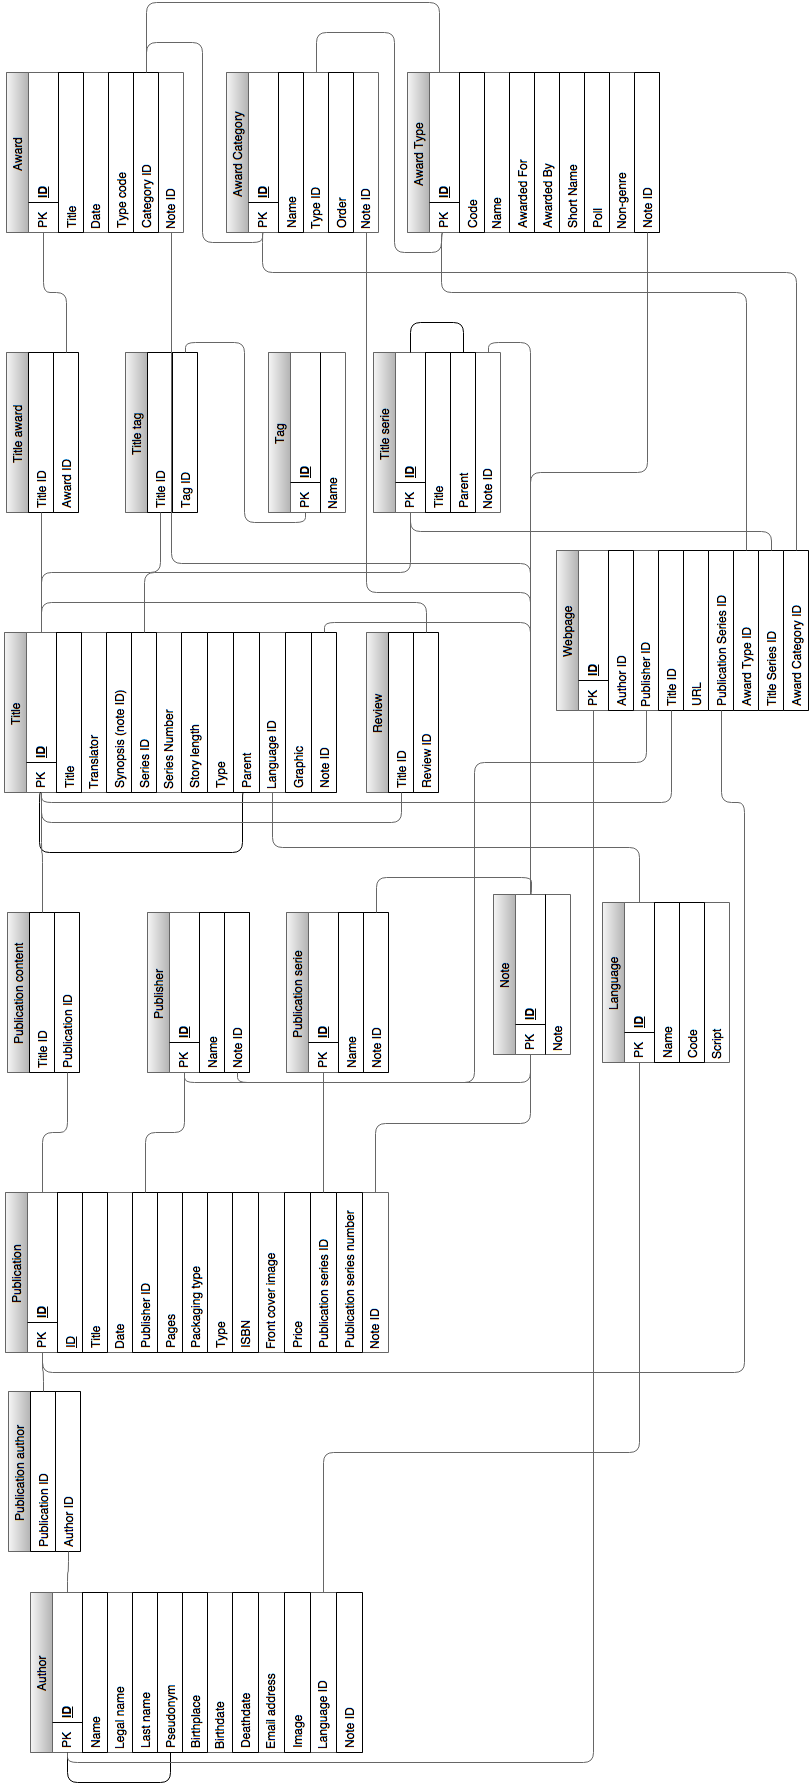
\includegraphics[scale = 0.33]{DBMS}
\end{center}

\newpage
\part{Delivrable 2}

\setcounter{section}{0}

\section{Modifications and improvements}

\subsection{Justifications}
We are now considering \texttt{award\char`_category} as a weak entity of \texttt{award\char`_type} since it doesn’t make sense for a category to exist without type. Therefore, the primary key of the category is now not only \texttt{cat\char`_ID} but also a tuple containing \texttt{cat\char`_ID} and \texttt{type\char`_ID}. This leads us to store again in our award table the \texttt{type\char`_ID} attribute to make the connection between awards and their categories.
\\
After analyzing the data, the graphic attribute may be null, we lead us to remove the NOT NULL constraint on this attribute.
\\
While inserting, we removed some of the notes entries due to bad formatting or empty content. Advanced data such as dates or combined page numbers have been parse the best possible. When that was not sufficient the field might have been replaced by null or replaced by the nearest value (e.g. 0/0/xxxx to 1/1/xxxx) as discussed in class. The translator field of titles has been extracted into a many to many relationship. The parser also been adapted to manage ‹ $\backslash\backslash$t › as an escape character for tabulation.
~\\~\\
In the DDL and according to the data, the following changes have been made :
\begin{itemize}
	\item \texttt{publisher\char`_id} in publication is now nullable
	\item \texttt{type} in publication is now nullable
	\item \texttt{parent} in titles is now nullable
	\item \texttt{url} in webpages is now not unique, as many url could reference different items
	\item \texttt{code} in \texttt{award\char`_type} is now not unique, as two awards could share the same initials
	\item drop table statements have been added to make easier the deletion and creation of the database
	\item dead foreign key values removal queries have been added to allow the creation of corresponding foreign keys
	\item a constraint ensuring at least of the entities is linked in each webpages entries has been added for not having a page referencing no entity
\end{itemize}
~\\
About cascade justifications, we decided with one of the TAs to only specify the behaviour for deleting as updating is not involved in the project. If not specified otherwise, we set the deleted field to null as they entities lifetime are independent of each others :
\begin{itemize}
	\item \texttt{authors\char`_id} and \texttt{pseudonym} are linked to the same person, thus requiring a cascade deletion.
	\item all many to many relationship have a cascade deletion, as there is no meaning of a two entity mapping missing one of the entity.
	\item \texttt{webpages} have a cascade deletion whenever one the referring entity is deleted.
	\item \texttt{awards\char`_categories} has a cascade deletion as it is a weak entity.
\end{itemize}
~\\
The enumerations values have been kept as inline values for flexibility and simplicity reasons as discussed with one of the teaching assistants. The full inserts are batched and executed in about 12 minutes.

\subsection{New ER Model}

\begin{center}
    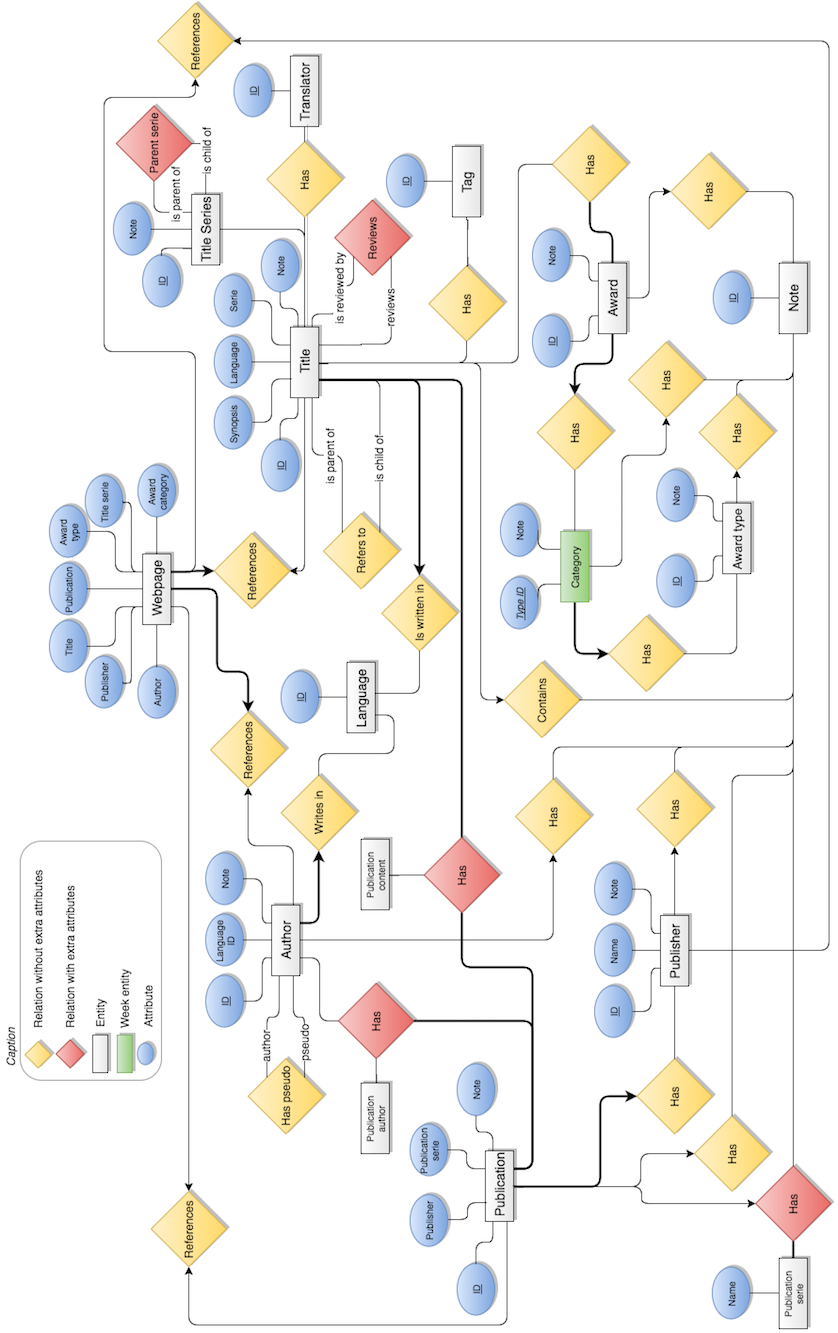
\includegraphics[scale = 0.5]{DBMS_ER_NEW}
\end{center}

\newpage
\section{Queries implementation}

\subsection{For every year, output the year and the number of publications for said year}
	\begin{enumerate}
	\item Description of logic : We are using the \texttt{DATE\char`_PART} function provided by Postgresql to extract the year of the date stored for each publication. Then
      we simply do a GROUP BY on the year and count the number of entries.
	\item SQL statement :
		\begin{lstlisting}[language=SQL,showspaces=false,basicstyle=\ttfamily,numberstyle=\tiny,commentstyle=\color{gray}]
SELECT DATE_PART('year', p.date_pub) AS year, COUNT(*) AS count
FROM publications p
GROUP BY DATE_PART('year', p.date_pub)
ORDER BY year ASC;
		\end{lstlisting}

	\item Results (partial):\\

	\begin{tabular}{|l|c|r|}
  \hline
  year & count \\
  \hline
2005 & 	8667\\
2006 & 	8166\\
2007 & 	11970\\
2008 & 	14204\\
2009 & 	15526\\
2010 & 	19150\\
2011 & 	22470\\
2012 & 	22317\\
2013 & 	22923\\
2014 & 	21219\\
2015 & 	17206\\
2016 & 	1590\\
8888 & 	445\\
9999 & 	4\\
\hline
\end{tabular}

	\end{enumerate}
	

\subsection{Output the names of the ten authors with most publications}

		\begin{enumerate}
	\item Description of logic : This query simply joins the authors and their publications and then GROUP BY on the author’s name. We just have to count the number of entries, ORDER BY that count and set a limit to 10.
	\item SQL statement :
		\begin{lstlisting}[language=SQL,showspaces=false,basicstyle=\ttfamily,numberstyle=\tiny,commentstyle=\color{gray}]
SELECT a.name, COUNT(*) AS count
FROM publications_authors p
INNER JOIN authors a ON p.author_id = a.id
GROUP BY a.name
ORDER BY count DESC
LIMIT 10;
		\end{lstlisting}

	\item Results :\\

	\begin{tabular}{|l|c|r|}
  \hline
  name & count \\
  \hline
uncredited & 2912\\
Isaac Asimov & 2389\\
Edgar Rice Burroughs & 2287\\
Robert A. Heinlein	& 1878\\
Arthur C. Clarke & 1512\\
Andre Norton & 1505\\
Stephen King & 1504\\
Robert Silverberg & 1481\\
Philip K. Dick & 1398\\
Terry Pratchett	& 1354\\
  \hline
\end{tabular}

	\end{enumerate}
\newpage

\subsection{What are the names of the youngest and oldest authors to publish something in 2010?}

			\begin{enumerate}
	\item Description of logic : Slightly more complicated this query uses nested subqueries to first select publications of 2010, then to select the maximum and minimum  birth dates of author that have some publication of 2010.
	\item SQL statement :
		\begin{lstlisting}[language=SQL,showspaces=false,basicstyle=\ttfamily,numberstyle=\tiny,commentstyle=\color{gray}]
SELECT a.name
FROM authors a
WHERE a.birth_date = (
SELECT MAX(a.birth_date) AS max
FROM publications_authors pa
JOIN authors a ON pa.author_id = a.id
WHERE pa.publication_id IN (
  SELECT pub.id
  FROM publications pub
  WHERE DATE_PART('year', pub.date_pub) = '2010'
)) OR
a.birth_date = (
SELECT MIN(a.birth_date) AS max
FROM publications_authors pa
JOIN authors A ON pa.author_id = a.id
WHERE pa.publication_id IN (
  SELECT pub.id
  FROM publications pub
  WHERE DATE_PART('year', pub.date_pub) = '2010'
));
		\end{lstlisting}

	\item Results :\\

	\begin{tabular}{|l|c|r|}
  \hline
  name \\
  \hline
Robert Henryson\\
Gavin Douglas\\
Greg Kurzawa\\
Laramie Sasseville\\
Brooke Vaughn\\
Pancham Yadav\\
Euripides\\
Aubrey Smith\\
Augustin Lardy\\
Livy\\
Michel Saint-Romain\\
Gan Bao\\
Timothy F. Mitchell\\
Gottfried von Strassburg\\
  \hline
\end{tabular}

	\end{enumerate}

\subsection{How many comics (graphic titles) have publications with less than 50 pages, less than 100 pages, and more (or equal) than 100 pages?}

	\begin{enumerate}
	\item Description of logic : After joining titles and publications, filtering them using the “graphic” field of titles and setting the condition on the number of pages, we just have to count the number of entries.
	\item SQL statement :
		\begin{lstlisting}[language=SQL,showspaces=false,basicstyle=\ttfamily,numberstyle=\tiny,commentstyle=\color{gray}]
SELECT COUNT(*)
FROM titles t
JOIN publications_contents AS pc ON t.id = pc.title_id
JOIN publications AS p ON pc.publication_id = p.id
WHERE t.graphic = 'YES'
AND p.Pages < 50;

------------------------------------------------

SELECT COUNT(*)
FROM titles t
JOIN publications_contents AS pc ON t.id = pc.title_id
JOIN publications AS p ON pc.publication_id = p.id
WHERE t.graphic = 'YES'
AND p.Pages < 100;

------------------------------------------------

SELECT COUNT(*)
FROM titles t
JOIN publications_contents AS pc ON t.id = pc.title_id
JOIN publications AS p ON pc.publication_id = p.id
WHERE t.graphic = 'YES'
AND p.Pages >= 100;
		\end{lstlisting}

	\item Results :\\

	\begin{tabular}{|l|c|r|}
	  \hline
		count \\
	  \hline
		153\\
	  \hline
	\end{tabular}

	\begin{tabular}{|l|c|r|}
	  \hline
		count \\
	  \hline
		202\\
	  \hline
	\end{tabular}

	\begin{tabular}{|l|c|r|}
	  \hline
		count \\
	  \hline
		194\\
	  \hline
	\end{tabular}

\end{enumerate}

\subsection{For every publisher, calculate the average price of its published novels (the ones that have a dollar price)}

	\begin{enumerate}
	\item Description of logic : This query joins the publications and authors via the \texttt{publications\char`_authors} table. Then it filters the publications to keep only the ones that have a price in dollar. Finally it groups everything on the author’s name and do an average on the price.
	\item SQL statement :
		\begin{lstlisting}[language=SQL,showspaces=false,basicstyle=\ttfamily,numberstyle=\tiny,commentstyle=\color{gray}]
ELECT pr.name, AVG(p.price) AS average
FROM publications p
JOIN publishers pr ON p.publisher_id = pr.id
WHERE p.currency = '$'
GROUP BY pr.name
ORDER BY average DESC;
		\end{lstlisting}

	\item Results (partial, 10 first):\\

	\begin{tabular}{|l|c|r|}
	  \hline
		  name & avg \\
	  \hline
		Library Fellows of the Whitney Museum of American Art & 2200\\
		The Pennyroyal Press & 1000\\
		Pickering \& Chatto & 795\\
		Epic Ink Books & 500\\
		The Book Club of California & 375\\
		Tradition Books & 357\\
		Charnel House & 344.88235294117646\\
		Subterranean Press \& PS Publishing & 300\\
		Sirius Science Fiction & 262.5\\
		Kluwer Academic Publishers & 259\\
	  \hline
\end{tabular}

\end{enumerate}

\subsection{What is the name of the author with the highest number of titles that are tagged as “science fiction”?}

	\begin{enumerate}
	\item Description of logic : This query use a subquery. This subquery links authors with their publications, the publications with their titles and finally the titles with their tags. A simple filter on tags to keep only the ones that have the keyword \texttt{sf} (meaning science fiction), then group by authors name, count the entries for each authors and order by this counter. Then the main query is there to keep the name without the counter.
	\item SQL statement :
		\begin{lstlisting}[language=SQL,showspaces=false,basicstyle=\ttfamily,numberstyle=\tiny,commentstyle=\color{gray}]
SELECT a.name
FROM authors a
JOIN (
	SELECT a.name AS n, COUNT(*) AS count_sf
	FROM authors a
	JOIN publications_authors pa ON a.id = pa.author_id
	JOIN publications p ON pa.publication_id = p.id
	JOIN publications_contents pc ON pc.publication_id = p.id
	JOIN titles t ON pc.title_id = t.id
	JOIN titles_tags tt ON t.id = tt.title_id
	JOIN tags ON tt.tag_id = tags.id
	WHERE tags.name '%science-fiction%'
	GROUP BY a.name
	ORDER BY count_sf DESC
	LIMIT 1)
c ON c.n = a.name;
		\end{lstlisting}

	\item Results :\\

	\begin{tabular}{|l|c|r|}
	  \hline
		name\\
	  \hline
		Maurice Level\\
	  \hline
	\end{tabular}
\end{enumerate}

\subsection{List the three most popular titles (i.e., the ones with the most awards and reviews)}

	\begin{enumerate}
	\item Description of logic : Here we order the titles on their number of awards and reviews and then simply sum them and order them on that total. Note that union is mandatory as otherwise we will miss some datas (e.g. all titles that only appear to have awards or titles).
	\item SQL statement :
		\begin{lstlisting}[language=SQL,showspaces=false,basicstyle=\ttfamily,numberstyle=\tiny,commentstyle=\color{gray}]
SELECT t.title, ts.count_awards + ts.count_reviews as total
FROM (
  SELECT ta.title_id, 0 AS count_reviews, COUNT(ta.award_id) AS count_awards
  FROM titles_awards ta
  GROUP BY ta.title_id
  UNION
  SELECT r.title_id, COUNT(r.review_id) AS count_reviews, 0 AS count_awards
  FROM reviews r
  GROUP BY r.title_id
) as ts
  INNER JOIN titles t on t.id = ts.title_id
ORDER BY total DESC
LIMIT 3;
		\end{lstlisting}

	\item Results :\\

	\begin{tabular}{|l|c|r|}
	  \hline
		title & total\\
	  \hline
		The Wonderful Wizard of Oz	& 100\\
		Sky Island	& 54\\
		The Sea Fairies	& 48\\
	  \hline
	\end{tabular}
\end{enumerate}

\newpage
\section{Interface}

\subsection{Screenshots}

\subsubsection{Menu}
\begin{figure}[!htb]
	\centering
    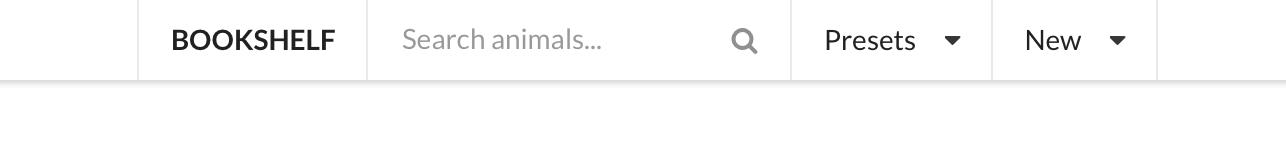
\includegraphics[scale = 0.5]{ui-menu}
    \caption{Menu view}
\end{figure}

\subsubsection{Selection}
\begin{figure}[!htb]
	\centering
    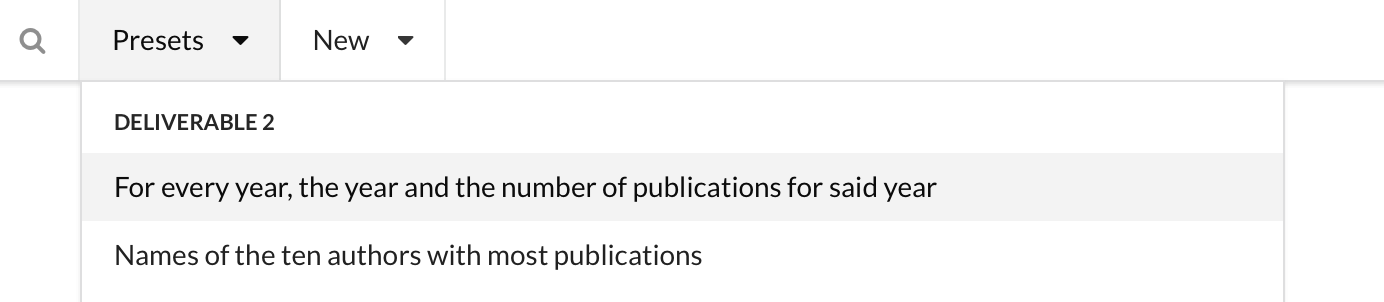
\includegraphics[scale = 0.5]{ui-selection}
    \caption{Selection view}
\end{figure}

\subsubsection{Preset}
\begin{figure}[!htb]
  \centering
  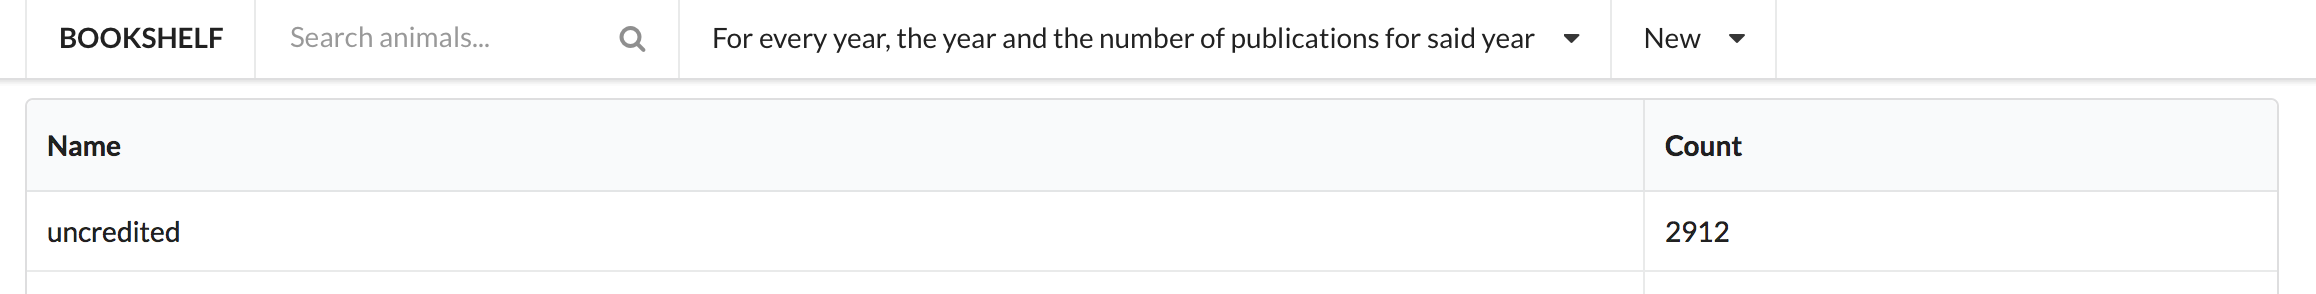
\includegraphics[scale = 0.45]{ui-preset}
  \caption{Preset view}
\end{figure}

\newpage

\subsubsection{Search}
\begin{figure}[!htb]
	\centering
    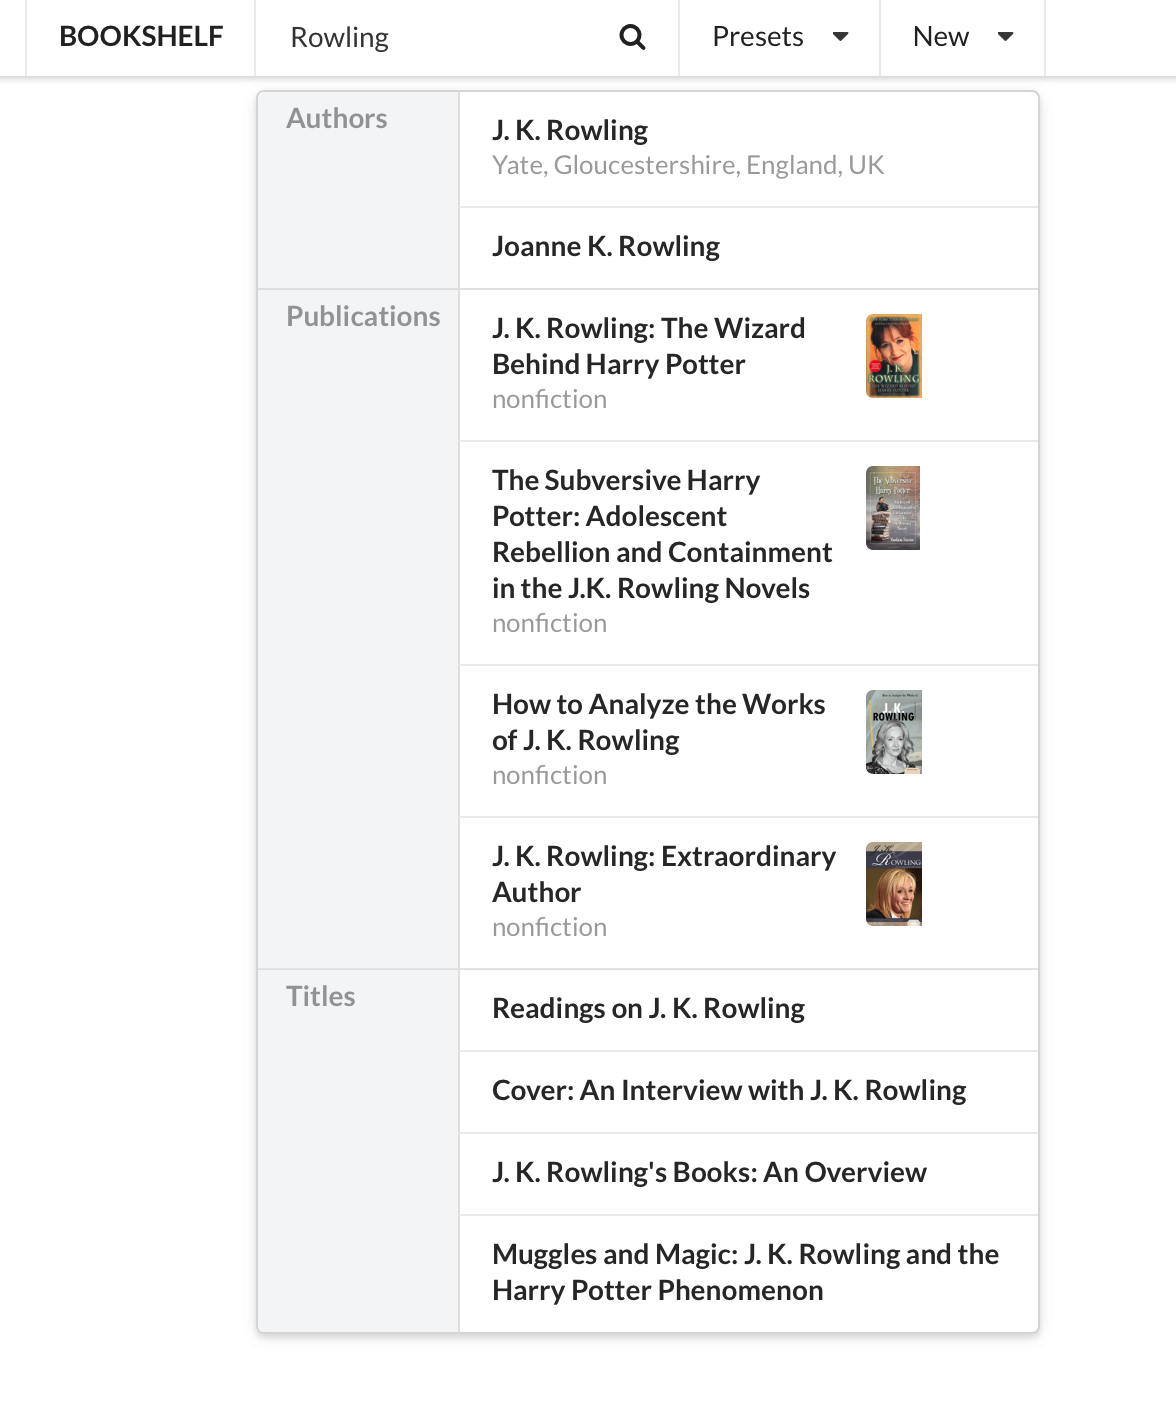
\includegraphics[scale = 0.4]{ui-search}
    \caption{Search view}
\end{figure}

\subsubsection{Insert}
\begin{figure}[!htb]
	\centering
    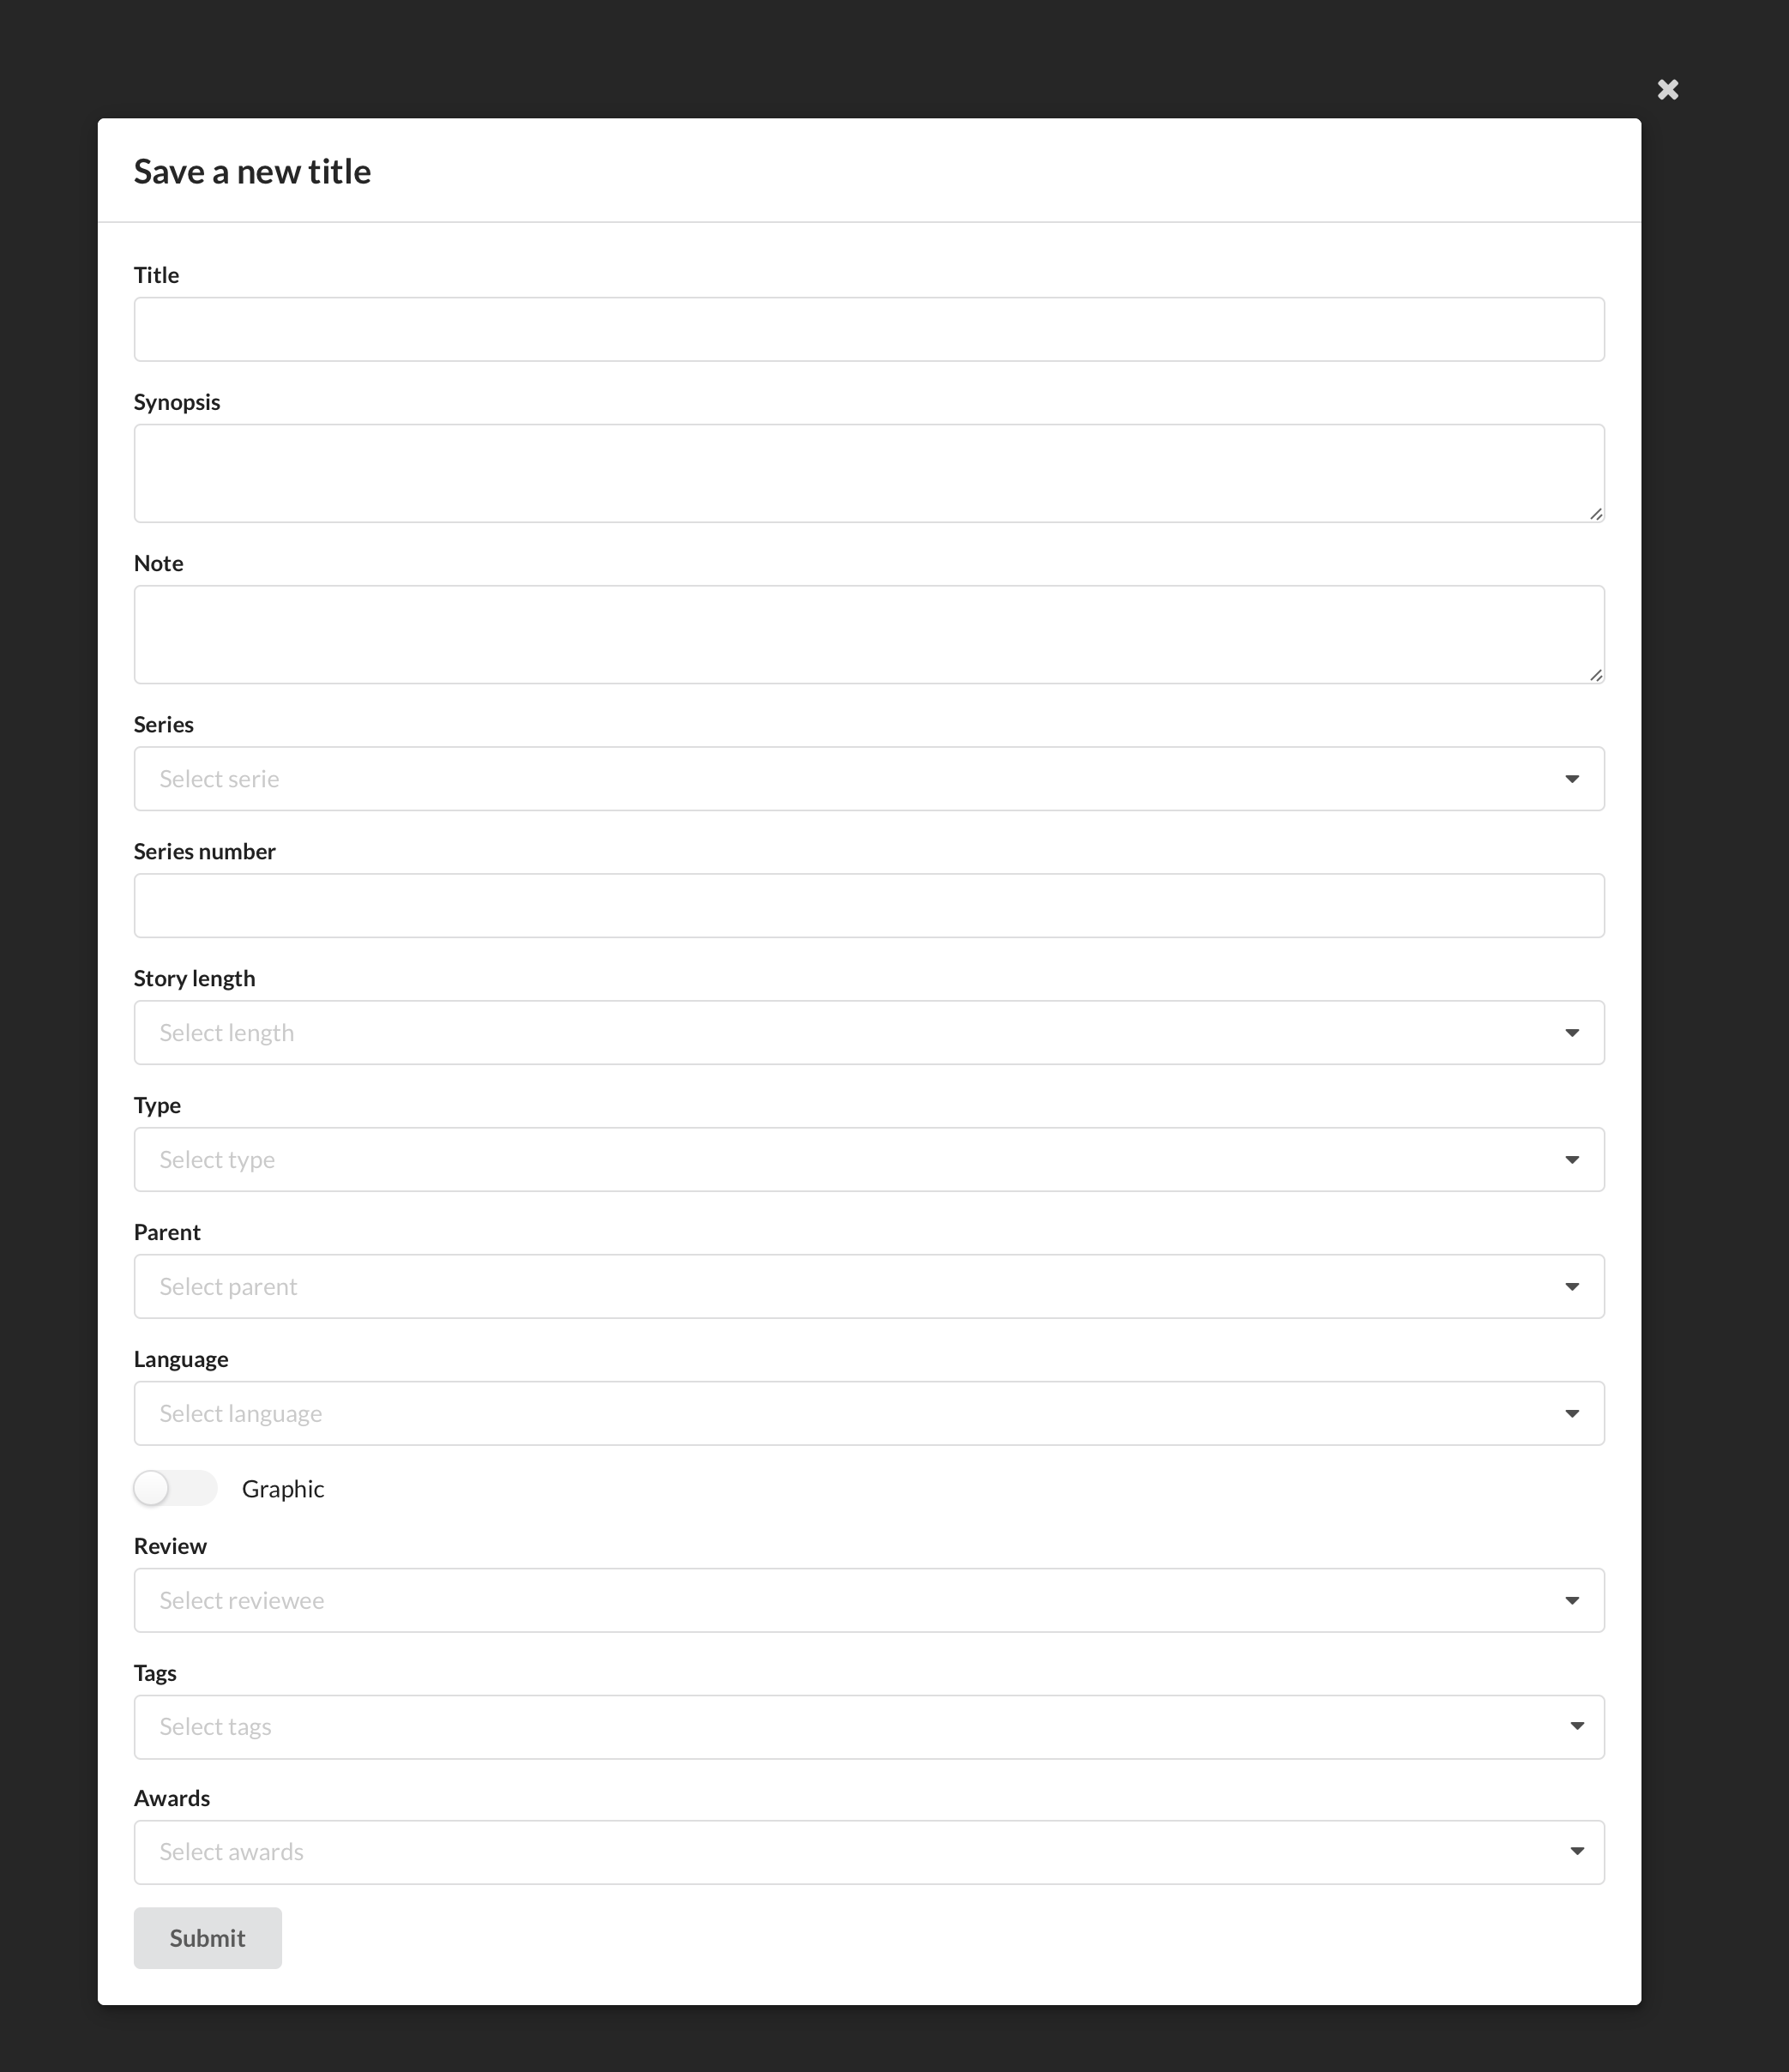
\includegraphics[scale = 0.25]{ui-insert}
    \caption{Insert view}
\end{figure}

\subsubsection{Result}
\begin{figure}[!htb]
	\centering
    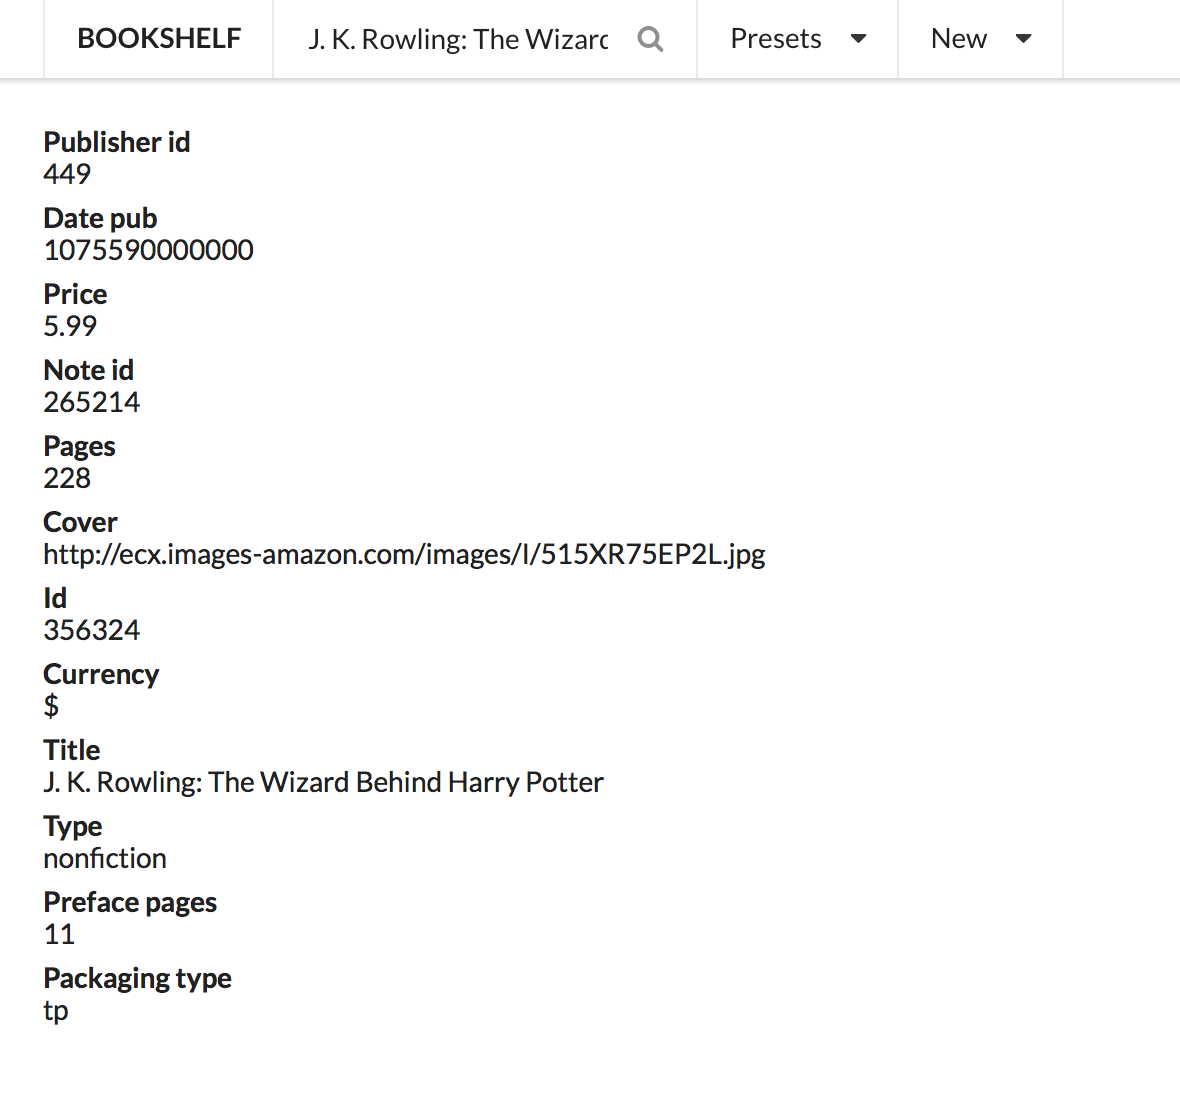
\includegraphics[scale = 0.5]{ui-result}
    \caption{Result view}
\end{figure}

\subsection{Implementation details}

The search field is using ajax to access our backend server in Scala (cf. search). For each search query, we run in parallel 3 queries using « LIKE » statements to find all relevant results and send it be aggregated to the requester. We limit the number of result to 4 for visibility reason. The user is able to always enter the main field (either name or title), a secondary field for more information about the entry (but not searchable) and optionally a picture of the entry if relevant. Once the entry is select more information about the result in a formatted way (cf. result).

\newpage
\part{Delivrable 3}

\setcounter{section}{0}

\section{Modifications and improvements}

\subsection{Justifications}
~\\
In the DDL and according to the data, the following changes have been made :
\begin{itemize}
	\item we replaced the \texttt{language} field by \texttt{language\char`_id} in \texttt{title\char`_translator} to be able to join this table with \texttt{language}.
\end{itemize}

\subsection{Query modifications}
~\\
As discussed in the feedback of our queries of deliverable 2, we also improve some queries :

\subsubsection{Output the names of the ten authors with most publications}

		\begin{enumerate}
	\item Modification done : following some advices, we replaced our previous query by this one using an inner query, to avoid an \texttt{INNER JOIN} over all authors.
	\item SQL statement :
		\begin{lstlisting}[language=SQL,showspaces=false,basicstyle=\ttfamily,numberstyle=\tiny,commentstyle=\color{gray}]
SELECT a.name
FROM authors a
WHERE a.id IN (
  SELECT p.author_id
  FROM publications_authors p
  GROUP BY p.author_id
  ORDER BY COUNT(p.author_id) DESC
  LIMIT 10
);
		\end{lstlisting}

\end{enumerate}

\subsubsection{What is the name of the author with the highest number of titles that are tagged as science fiction}

	\begin{enumerate}
	\item Modification done : our \texttt{LIKE} tag is now stronger to fit the data, and we also remove some unnecessary joins for the purpose of this query.
	\item SQL statement :
		\begin{lstlisting}[language=SQL,showspaces=false,basicstyle=\ttfamily,numberstyle=\tiny,commentstyle=\color{gray}]
SELECT a.name
FROM authors a
  INNER JOIN publications_authors pa ON a.id = pa.author_id
  INNER JOIN publications_contents pc ON pc.publication_id = pa.publication_id
  INNER JOIN titles_tags tt ON pc.title_id = tt.title_id
  INNER JOIN tags ON tt.tag_id = tags.id
WHERE tags.name LIKE '%science fiction%'
GROUP BY a.name
ORDER BY COUNT(DISTINCT pc.title_id) DESC
LIMIT 1;
		\end{lstlisting}

\end{enumerate}

\newpage

\subsubsection{List the three most popular titles (i.e., the ones with the most awards and reviews)}

	\begin{enumerate}
	\item Modification done : something went wrong while copying the query into this report to the point results were not matching the query as it was underlying in the feedback. This time, the above query behaves exactly as we are expecting, and outputs only title once, by summing them if needed.
	\item SQL statement :
		\begin{lstlisting}[language=SQL,showspaces=false,basicstyle=\ttfamily,numberstyle=\tiny,commentstyle=\color{gray}]
SELECT t.title
FROM titles t
  LEFT OUTER JOIN titles_awards ta ON ta.title_id = t.id
  LEFT OUTER JOIN reviews r ON r.title_id = t.id
GROUP BY t.id, t.title
ORDER BY COUNT(DISTINCT ta.award_id) + COUNT(DISTINCT r.review_id) DESC
LIMIT 3;
		\end{lstlisting}

\end{enumerate}
~\\
We've also modified also queries that were counting something, by replacing \texttt{COUNT(*)} by \texttt{COUNT(id)} for instance to be more precise and know exactly what we were indeed counting (we also wanted to remove null values, but in this example it is not likely going to happen since it is a primary key).

\section{Queries implementation}

Note that we are not using an Oracle server but our own one, running with \texttt{Postgres SQL}. Therefore, some queries may contain some syntax that are specific to it.

\subsection{Compute the average price per currency of the publications of the most popular title (i.e, the title with most publications overall)}
	\begin{enumerate}
	\item Description of logic : This query relies on a join between \texttt{publications} and \texttt{publications\char`_contents}, where the most popular title is determined by grouping publications by \texttt{title\char`_id}, counting them in descendant and just take the first result. Therefore, our nested query is simply called with an \texttt{=}. We also remove null values to not skew results, and take at the end the average for each currency.
	\item SQL statement :
		\begin{lstlisting}[language=SQL,showspaces=false,basicstyle=\ttfamily,numberstyle=\tiny,commentstyle=\color{gray}]
SELECT
  AVG(p.price),
  p.currency
FROM publications p
  JOIN publications_contents pc ON p.id = pc.publication_id
WHERE
  pc.title_id = (
    SELECT pc.title_id
    FROM publications_contents pc
    GROUP BY pc.title_id
    ORDER BY COUNT(pc.publication_id) DESC
    LIMIT 1
  )
  AND p.currency IS NOT NULL
GROUP BY p.currency;
		\end{lstlisting}

	\item Results :\\

	\begin{tabular}{|l|c|r|}
  \hline
  avg & currency \\
  \hline
5.713500000000002	& \pounds \\
7.784824120603027	& \$ \\
\hline
\end{tabular}

	\end{enumerate}
	

\subsection{Output the names of the top ten title series with most awards}

		\begin{enumerate}
	\item Description of logic : the logic of this query is, in a sense, the same as the previous one, excepting that we don't need any nested query. Grouping by title and associate to them their award counts allow us to achieve what is asking.
	\item SQL statement :
		\begin{lstlisting}[language=SQL,showspaces=false,basicstyle=\ttfamily,numberstyle=\tiny,commentstyle=\color{gray}]
SELECT ts.title
FROM titles t
  JOIN titles_awards ta ON t.id = ta.title_id
  JOIN titles_series ts ON t.series_id = ts.id
WHERE t.series_id IS NOT NULL
GROUP BY ts.title
ORDER BY COUNT(ta.award_id) DESC
LIMIT 10;
		\end{lstlisting}

	\item Results :\\

	\begin{tabular}{|l|c|r|}
  \hline
  title \\
  \hline
Science Fact (Analog) \\
Tor.com \\
Hainish \\
Locus \\
Kirinyaga \\
Miles Vorkosigan \\
Newford \\
The Year's Best Fantasy and Horror \\
Science Fiction Chronicle \\
Book of The New Sun \\
  \hline
\end{tabular}

	\end{enumerate}

\subsection{Output the name of the author who has received the most awards after his/her death}

			\begin{enumerate}
	\item Description of logic : joining tables is the keyword for this query, following our ER model, to go from author to his associated awards, we need to go through 5 different tables (so, it means 4 joins). Once this is done, we simply need to precise the condition \textit{award received after his death}, and we take the initiative to also remove null values to avoid surprises. Eventually, to get only one author, we group them, and simply order them by their number of awards where, once again, we take the first result.
	\item SQL statement :
		\begin{lstlisting}[language=SQL,showspaces=false,basicstyle=\ttfamily,numberstyle=\tiny,commentstyle=\color{gray}]
SELECT a.name
FROM authors a
  JOIN publications_authors pa ON a.id = pa.author_id
  JOIN publications_contents pc ON pa.publication_id = pc.publication_id
  JOIN titles_awards ta ON pc.title_id = ta.title_id
  JOIN awards aw ON ta.award_id = aw.id
WHERE
  a.death_date IS NOT NULL
  AND aw.date > a.death_date
GROUP BY a.name
ORDER BY COUNT(ta.award_id) DESC
LIMIT 1;
		\end{lstlisting}

	\item Results :\\

	\begin{tabular}{|l|c|r|}
  \hline
  name \\
  \hline
H. G. Wells\\
  \hline
\end{tabular}

	\end{enumerate}

\subsection{For a given year, output the three publishers that published the most publications}

	\begin{enumerate}
	\item Description of logic : this query is parametrised and takes an input, which means the need of a \texttt{?} in the query that, once executed, will be replaced by the input of the user. This query is easy as it only relies on one join, no more explanation are therefore needed.
	\item SQL statement :
		\begin{lstlisting}[language=SQL,showspaces=false,basicstyle=\ttfamily,numberstyle=\tiny,commentstyle=\color{gray}]
SELECT p.name
FROM publishers p
  JOIN publications pu ON p.id = pu.publisher_id
WHERE DATE_PART('year', pu.date_pub) = ?
GROUP BY p.name
ORDER BY COUNT(DISTINCT pu.id) DESC
LIMIT 3;
		\end{lstlisting}

	\item Results :
	\begin{itemize}
	\item For 1982 :~\\~\\
	\begin{tabular}{|l|c|r|}
	  \hline
		name \\
	  \hline
		Ace Books\\
		Del Rey / Ballantine\\
		Berkley Books\\
	  \hline
	\end{tabular}
	\item For 2015 :~\\~\\
	\begin{tabular}{|l|c|r|}
	  \hline
		name \\
	  \hline
		CreateSpace\\
		Tor\\
		Open Road Integrated Media\\
	  \hline
	\end{tabular}
	\end{itemize}
\end{enumerate}

\subsection{Given an author, compute his/her most reviewed title(s)}

	\begin{enumerate}
	\item Description of logic : the \texttt{?} presence is for the same reason as before. According to our ER model, from authors to reviews, we need 5 different tables. Once joins done, we group our results by id and count the number of (previously joined) associated reviews.
	\item SQL statement :
		\begin{lstlisting}[language=SQL,showspaces=false,basicstyle=\ttfamily,numberstyle=\tiny,commentstyle=\color{gray}]
SELECT t.title
FROM authors a
  INNER JOIN publications_authors pa ON pa.author_id = a.id
  INNER JOIN publications_contents pc ON pc.publication_id = pa.publication_id
  INNER JOIN titles t ON t.id = pc.title_id
  INNER JOIN reviews r ON r.title_id = t.id
WHERE a.id = ?
GROUP BY t.id
ORDER BY COUNT(DISTINCT r.review_id) DESC;
		\end{lstlisting}

	\item Results :
	\begin{itemize}
	\item For id = 3123 : ~\\~\\
	\begin{tabular}{|l|c|r|}
	  \hline
		title \\
	  \hline
		The Search for Happily-Ever-After\\
	  \hline
	\end{tabular}
	\item For id = 123456 :~\\~\\
	\begin{tabular}{|l|c|r|}
	  \hline
		title \\
	  \hline
		Trick Cinematography: The Oscar Special-Effects Movies\\
	  \hline
	\end{tabular}
	\end{itemize}
\end{enumerate}

\subsection{For every language, find the top three title types with most translations}

	\begin{enumerate}
	\item Description of logic : After doing the cross product of all titles, languages and translations, we group over title type and then sort them according to their ids. Furthermore, in each of this group, we group them by language using \texttt{PARTITION BY}, and sort them according to the same rule, that allows us to number results by row number to eventually limit the output to 3 results by language by taking only the row whose number is less or equal than 3.
	\item SQL statement :
		\begin{lstlisting}[language=SQL,showspaces=false,basicstyle=\ttfamily,numberstyle=\tiny,commentstyle=\color{gray}]
SELECT
  r.name,
  r.type
FROM (
       SELECT
         l.name,
         t.type,
         ROW_NUMBER() OVER 
             (PARTITION BY l.id ORDER BY COUNT(DISTINCT t.id) DESC) as row
       FROM languages l
         INNER JOIN titles_translators tt ON tt.language_id = l.id
         INNER JOIN titles t ON tt.title_id = t.id
       GROUP BY t.type, l.name, l.id
       ORDER BY COUNT(DISTINCT t.id) DESC
     ) r
WHERE r.row <= 3;
		\end{lstlisting}

	\item Results :\\

	\begin{tabular}{|l|c|r|}
	  \hline
		name & type\\
	  \hline
		English	& shortfiction \\
		English	& serial \\
		English	& poem \\
		Italian	& novel \\
		Romanian & novel \\
		Russian	& novel \\
	  \hline
	\end{tabular}
\end{enumerate}

\subsection{For each year, compute the average number of authors per publisher}

	\begin{enumerate}
	\item Description of logic : we are using a nested query that outputs the name of the publisher, the year taken into consideration and the number of authors for that given year. Using such a nested query is required here as we are eager to get the average number of authors, therefore, the inner return return the count and the publisher, the outer one group them according to the year and compute the average.
	\item SQL statement :
		\begin{lstlisting}[language=SQL,showspaces=false,basicstyle=\ttfamily,numberstyle=\tiny,commentstyle=\color{gray}]
SELECT
  r.name,
  r.year,
  AVG(r.count)
FROM (
       SELECT DISTINCT
         pr.name,
         DATE_PART('year', p.date_pub) AS year,
         COUNT(DISTINCT pa.author_id) as count
       FROM publications p
         INNER JOIN publications_authors pa ON pa.publication_id = p.id
         INNER JOIN publishers pr ON pr.id = p.publisher_id
       GROUP BY pr.id, p.date_pub
     ) r
GROUP BY r.year, r.name;
		\end{lstlisting}

	\item Results (partial for year 2016) :\\

	\begin{tabular}{|l|c|r|}
	  \hline
		name & year & avg\\
	  \hline
		BBC Books &	2016 & 1.5\\
		Berkley Books & 2016 & 3.5\\
		Black Library / BL Publishing (UK) & 2016 & 2\\
		Black Swan & 2016 & 1\\
		Blanvalet & 2016 & 1.5\\
		Blink & 2016 & 1\\
		Bloomsbury Academic	& 2016 & 1\\
		Bloomsbury Children's Books (UK) & 2016	& 1.5\\
		Bloomsbury Circus & 2016 & 1\\
	  \hline
	\end{tabular}
\end{enumerate}

\subsection{Find the publication series with most titles that have been given awards of “World Fantasy Award” type}

	\begin{enumerate}
	\item Description of logic : we are mapping publication series to their award, this requires to join with other tables such as \texttt{publications}, \texttt{publications\char`_contents}, \texttt{titles\char`_awards}, \texttt{awards} and \texttt{awards\char`_types}. Once done, we taken the condition "type of award = world fantasy". Grouping and then ordering by title gives us the expected result.
	\item SQL statement :
		\begin{lstlisting}[language=SQL,showspaces=false,basicstyle=\ttfamily,numberstyle=\tiny,commentstyle=\color{gray}]
SELECT ps.name
FROM publications_series ps
  INNER JOIN publications p ON p.pub_series_id = ps.id
  INNER JOIN publications_contents pc ON pc.publication_id = p.id
  INNER JOIN titles_awards ta ON  ta.title_id = pc.title_id
  INNER JOIN awards a ON a.id = ta.award_id
  INNER JOIN awards_types at ON at.id = a.type_id
WHERE at.name = 'World Fantasy Award'
GROUP BY ps.id
ORDER BY COUNT(DISTINCT pc.title_id) DESC;
		\end{lstlisting}

	\item Results (partial, first ten) :\\

	\begin{tabular}{|l|c|r|}
	  \hline
		name \\
	  \hline
		DAW Collectors\\
		Golden Gryphon\\
		Millennium / Gollancz Fantasy Masterworks\\
		Fantasy Masterworks (II)\\
		SF Gateway Omnibus\\
		Signed First Editions of Science Fiction\\
		A Tor.com Original\\
		SFBC 50th Anniversary Collection\\
		Spectra Special Editions\\
		Open Road Media Sci-Fi \& Fantasy\\
	  \hline
	\end{tabular}
\end{enumerate}

\newpage

\subsection{For every award category, list the names of the three most awarded authors}

	\begin{enumerate}
	\item Description of logic : The nested query behaves more a less as the 6th one. This also outputs the count of awards. The outer query ensures this time on one hand to limit the number of results and on the other hand to return the name of the award as tis category. Note that results may sound incorrect (more than 3 results per category) but in fact they are correct since some category have some similar names.
	\item SQL statement :
		\begin{lstlisting}[language=SQL,showspaces=false,basicstyle=\ttfamily,numberstyle=\tiny,commentstyle=\color{gray}]
SELECT
  r.name,
  r.cat_name
FROM (
       SELECT
         a.name,
         ac.name AS cat_name,
         COUNT(DISTINCT aw.id) as count,
         ROW_NUMBER() OVER 
             (PARTITION BY ac.id ORDER BY COUNT(DISTINCT aw.id) DESC) AS row
       FROM awards_categories ac
         INNER JOIN awards aw ON aw.category_id = ac.id
         INNER JOIN titles_awards ta ON ta.award_id = aw.id
         INNER JOIN publications_contents pc ON pc.title_id = ta.title_id
         INNER JOIN publications_authors pa 
         	ON pa.publication_id = pc.publication_id
         INNER JOIN authors a ON a.id = pa.author_id
       GROUP BY a.name, cat_name, ac.id, a.id
       ORDER BY count DESC
     ) r
WHERE r.row <= 3;
		\end{lstlisting}

	\item Results (partial, first ten results) :\\

	\begin{tabular}{|l|c|r|}
	  \hline
		name & cat name \\
	  \hline
Gardner Dozois	& Best Novelette\\
Gardner Dozois	& Best Short Story\\
Gardner Dozois	& Best Novella\\
Gardner Dozois	& Best Short Story\\
Gardner Dozois	& Best Novelette\\
Gardner Dozois	& Best Novelette\\
Gardner Dozois	& Best Novella\\
Stanley Schmidt	& Best Short Story\\
Ellen Datlow	& Best Short Story\\
Gardner Dozois	& Best Novella\\
	  \hline
	\end{tabular}
\end{enumerate}

\subsection{Output the names of all living authors that have published at least one anthology from youngest to oldest}

	\begin{enumerate}
	\item Description of logic : this query is simple and behaves exactly as ones previously written. We simply do some joins, and then apply the conditions. Eventually, we order the results by their birth date.
	\item SQL statement :
		\begin{lstlisting}[language=SQL,showspaces=false,basicstyle=\ttfamily,numberstyle=\tiny,commentstyle=\color{gray}]
SELECT DISTINCT a.name, a.birth_date
FROM authors a
  INNER JOIN publications_authors pa ON pa.author_id = a.id
  INNER JOIN publications p ON p.id = pa.publication_id
  INNER JOIN publications_contents pc ON pc.publication_id = p.id
  INNER JOIN titles t ON t.id = pc.title_id
WHERE
  t.type = 'anthology'
  AND a.death_date IS NULL
  AND a.birth_date IS NOT NULL
ORDER BY a.birth_date DESC;
		\end{lstlisting}

	\item Results :\\

	\begin{tabular}{|l|c|r|}
	  \hline
		name & birth date (yyyy-MM-dd)\\
	  \hline
Stefan Bachmann	& 1993-01-01\\
Brit Mandelo	& 1990-05-13\\
Brandon Rospond	& 1989-03-24\\
Monique Snyman	& 1988-09-27\\
Kasey Lansdale	& 1988-06-24\\
Cameron Pierce	& 1988-05-23\\
Chris Kelso	& 1988-03-22\\
Cody Martin	& 1987-02-10\\
Bethany Zaiatz	& 1987-01-01\\
Steve Mollmann	& 1985-07-10\\
	  \hline
	\end{tabular}
\end{enumerate}

\subsection{Compute the average number of publications per publication series (single result/number expected)}

	\begin{enumerate}
	\item Description of logic : we previously met the case where we wanted an average of a group. We achieved this by using a nested query that is grouping its result on something and outputs the count of these. Then, the outer query needs simply to take the result and do the average as it is already a count.
	\item SQL statement :
		\begin{lstlisting}[language=SQL,showspaces=false,basicstyle=\ttfamily,numberstyle=\tiny,commentstyle=\color{gray}]
SELECT AVG(count.ncount)
FROM (
       SELECT COUNT(ps.name) as ncount
       FROM publications p
         INNER JOIN publications_series ps ON ps.id = p.pub_series_id
       GROUP BY ps.name
     ) count;
		\end{lstlisting}

	\item Results :\\

	\begin{tabular}{|l|c|r|}
	  \hline
		avg\\
	  \hline
		12.1544117647058824\\
	  \hline
	\end{tabular}
\end{enumerate}

\subsection{Find the author who has reviewed the most titles}

	\begin{enumerate}
	\item Description of logic : we are using here a nested query for efficiency purposes as we know we only want one result and so don't want to join informations with authors that do not respect the condition. This nested query returns the id of the author who has reviewed most titles, by taking only titles with the type 'review', grouping them by \texttt{author\char`_id}, and counting the number of titles.
	\item SQL statement :
		\begin{lstlisting}[language=SQL,showspaces=false,basicstyle=\ttfamily,numberstyle=\tiny,commentstyle=\color{gray}]
SELECT a.name
FROM authors a
WHERE a.id = (
  SELECT pa.author_id
  FROM publications p
    INNER JOIN publications_authors pa ON pa.publication_id = p.id
    INNER JOIN publications_contents pc ON pc.publication_id = p.id
    INNER JOIN titles t ON t.id = pc.title_id
  WHERE t.type = 'review'
  GROUP BY pa.author_id
  ORDER BY COUNT(DISTINCT pc.title_id) DESC
  LIMIT 1
);
		\end{lstlisting}

	\item Results :\\

	\begin{tabular}{|l|c|r|}
	  \hline
		name\\
	  \hline
		Charles N. Brown\\
	  \hline
	\end{tabular}
\end{enumerate}

\subsection{For every language, list the three authors with the most translated titles of “novel” type}

	\begin{enumerate}
	\item Description of logic : This query behaves exactly as the ninth one, except that we are not dealing with award but with author this time.
	\item SQL statement :
		\begin{lstlisting}[language=SQL,showspaces=false,basicstyle=\ttfamily,numberstyle=\tiny,commentstyle=\color{gray}]
SELECT
  r.name,
  r.auth_name
FROM (
       SELECT DISTINCT
         l.name,
         l.id,
         a.name AS auth_name,
         COUNT(DISTINCT t.id) AS count,
         ROW_NUMBER() OVER
         	(PARTITION BY l.id ORDER BY COUNT(DISTINCT t.id) DESC) as row
       FROM languages l
         INNER JOIN titles_translators tt ON tt.language_id = l.id
         INNER JOIN titles t ON tt.title_id = t.id
         INNER JOIN publications_contents pc ON pc.title_id = t.id
         INNER JOIN publications_authors pa
         	ON pa.publication_id = pc.publication_id
         INNER JOIN authors a ON a.id = pa.author_id
       WHERE t.type = 'novel'
       GROUP BY l.id, l.name, a.id, a.name
       ORDER BY count DESC
     ) r
WHERE r.row <= 3;
		\end{lstlisting}

	\item Results :\\

	\begin{tabular}{|l|c|r|}
	  \hline
		name & auth name\\
	  \hline
English	& Robert Merle\\
English	& Mikhail Bulgakov\\
English	& Stanisław Lem\\
Italian	& Greg Egan\\
Romanian & Greg Egan\\
Russian	& Arkady Strugatsky\\
Russian	& Boris Strugatsky\\
	  \hline
	\end{tabular}
\end{enumerate}

\newpage

\subsection{Order the top ten authors whose publications have the largest pages per dollar ratio (considering all publications of an author that have a dollar price)}

	\begin{enumerate}
	\item Description of logic : the need of an inner query is for the same reason described in the previous query. The only difference is that this time we do not use a \texttt{FROM} to join our inner query but a \texttt{JOIN} as we do not want to only one result. The inner query join publications to their author since we are interesting in authors. Furthermore, the \texttt{WHERE} clause ensures that publications have a dollar price, and price are not equal to zero (hence, not NULL too) to avoid division by zero. Eventually, we group this by \texttt{author\char`_id}, \texttt{price} and \texttt{pages}, and order by the ratio $\frac{pages}{price}$, limiting the results to ten.
	\item SQL statement :
		\begin{lstlisting}[language=SQL,showspaces=false,basicstyle=\ttfamily,numberstyle=\tiny,commentstyle=\color{gray}]
SELECT a.name
FROM authors a
  INNER JOIN (
    SELECT pa.author_id
    FROM publications p
      INNER JOIN publications_authors pa ON pa.publication_id = p.id
    WHERE
      p.currency = '$'
      AND p.pages != 0
      AND p.price != 0
      GROUP BY pa.author_id, p.price, p.pages
      ORDER BY p.pages / p.price DESC
      LIMIT 10
	) AS paa ON paa.author_id = a.id;
		\end{lstlisting}

	\item Results :\\

	\begin{tabular}{|l|c|r|}
	  \hline
		name\\
	  \hline
Hugh Lofting\\
Debra Doyle\\
James D. Macdonald\\
John W. Campbell, Jr.\\
Frank Baum\\
Victor Appleton\\
H. Beam Piper\\
Meredith Badger\\
Evelyn Kriete\\
John Gregory Betancourt\\
	  \hline
	\end{tabular}
\end{enumerate}

\newpage

\subsection{For publications that have been awarded the Nebula award, find the top 10 with the most extensive web presence  (i.e, the highest number of author websites, publisher websites, publication series websites, and title series websites in total)}

	\begin{enumerate}
	\item Description of logic : this query requires a lot of workload as it relies in a way on all tables so we will need to join our initial table (webpage as we are looking for web presence). The \texttt{INNER JOIN} takes care to only join needed rows and uses a quite different syntax with \texttt{ON ... OR ...} to allow joining with a table potentially only one key that interests us. Eventually, we group this in the outer query by \texttt{publication\char`_id} and \texttt{title}, and order all this by the sum of what is interesting us here (see below).
	\item SQL statement :
		\begin{lstlisting}[language=SQL,showspaces=false,basicstyle=\ttfamily,numberstyle=\tiny,commentstyle=\color{gray}]
SELECT r.title
FROM webpages w
  INNER JOIN (
    SELECT DISTINCT
      pc.publication_id AS publication_id,
      ps.id AS publications_series_id,
      p2.id AS publisher_id,
      pa.author_id AS author_id,
      ts.id AS title_series_id,
      p.title AS title
     FROM publications_contents pc
     INNER JOIN publications p ON p.id = pc.publication_id
     INNER JOIN publishers p2 ON p2.id = p.publisher_id
     INNER JOIN titles t ON t.id = pc.title_id
     INNER JOIN titles_series ts ON ts.id = t.series_id
     INNER JOIN publications_series ps ON ps.id = p.pub_series_id
     INNER JOIN publications_authors pa ON pa.publication_id = pc.publication_id
     INNER JOIN titles_awards ta ON ta.title_id = pc.title_id
     INNER JOIN awards a ON a.id = ta.award_id
     INNER JOIN awards_types at ON at.id = a.type_id
     WHERE at.name = 'Nebula Award'
    ) AS r ON r.author_id = w.author_id
           OR r.publisher_id = w.publisher_id
           OR r.publications_series_id = w.publications_series_id
           OR r.title_series_id = w.title_series_id
GROUP BY (r.publication_id, r.title)
ORDER BY
  COUNT(DISTINCT r.author_id)
  + COUNT(DISTINCT r.publisher_id)
  + COUNT(DISTINCT r.publications_series_id)
  + COUNT(DISTINCT r.title_series_id) DESC
LIMIT 10;
		\end{lstlisting}

	\item Results :\\

	\begin{tabular}{|l|c|r|}
	  \hline
		title\\
	  \hline
Novel Ideas: Fantasy\\
The Saturn Game / Iceborn\\
13 Short Science Fiction Novels\\
13 Short Fantasy Novels\\
A Meeting with Medusa / Green Mars\\
Fugue State / The Death of Doctor Island\\
Future Earths: Under African Skies\\
Explorations\\
Born With the Dead / The Saliva Tree\\
The 1983 Annual World's Best SF\\
	  \hline
	\end{tabular}
\end{enumerate}

\newpage

\section{Queries optimization}

\subsection{Query 1 : Output the name of the author who has received the most awards after his/her death}

\subsubsection{Query}
		\begin{lstlisting}[language=SQL,showspaces=false,basicstyle=\ttfamily,numberstyle=\tiny,commentstyle=\color{gray}]
SELECT a.name
FROM authors a
  JOIN publications_authors pa ON a.id = pa.author_id
  JOIN publications_contents pc ON pa.publication_id = pc.publication_id
  JOIN titles_awards ta ON pc.title_id = ta.title_id
  JOIN awards aw ON ta.award_id = aw.id AND aw.date > a.death_date
WHERE a.death_date IS NOT NULL
GROUP BY a.name
ORDER BY COUNT(ta.award_id) DESC
LIMIT 1;
		\end{lstlisting}
~\\	
This query basically links the tables `authors` and `awards` by doing multiple joins with tables in between. Then it simply checks if the author is dead and filter to keep only the awards that has been received after his death. Finally we order the final results on the number of awards remaining per author and keep only the first result, the one with most award. The \texttt{AND} clause is now in the join to allow less joins.~\\
		
\subsubsection{Running time \& optimization}

The query runs in approximately \textbf{700ms}. This time is mainly distributed between the full scans of tables and joins. We already spent 99.96\% of the time when the joins are done. So even if we create an index on fields used in the where clauses or aggregate actions, we won't see any improvement.

\subsubsection{Plan}
The plan for query 12 is simple to understand. We see that it first does the join between \texttt{authors} and ~\\ \texttt{publications\char`_authors} then joins the resulting table with \texttt{publications\char`_contents}, same thing for \texttt{titles\char`_awards} and finally \texttt{awards}. At this point we still have 3987 rows. The aggregate operation is simply the \texttt{COUNT}, then the sort is on `a.name` and the limit keeps only one result.
We can see that the time after the joins is 59997 and at the end of the execution 60017. The time of the joins highly depends on the number of processed rows.

\begin{figure}[!htb]
	\centering
    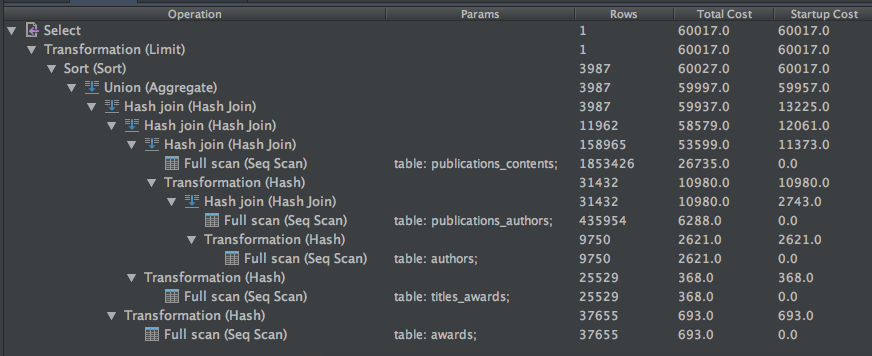
\includegraphics[scale = 0.5]{./query_analysis/query12}
    \caption{Running plan for this query (obtained with Datagrip)}
\end{figure}


\subsection{Query 2 : For each year, compute the average number of authors per publisher}

\subsubsection{Initial query}
		\begin{lstlisting}[language=SQL,showspaces=false,basicstyle=\ttfamily,numberstyle=\tiny,commentstyle=\color{gray}]
SELECT
  r.name,
  r.year,
  AVG(r.count)
FROM (
       SELECT DISTINCT
         pr.name,
         DATE_PART('year', p.date_pub) AS year,
         COUNT(DISTINCT pa.author_id) as count
       FROM publications p
         INNER JOIN publications_authors pa ON pa.publication_id = p.id
         INNER JOIN publishers pr ON pr.id = p.publisher_id
       GROUP BY pr.id, p.date_pub
     ) r
GROUP BY r.year, r.name;
		\end{lstlisting}
~\\	
This query uses a subquery for it's \texttt{FROM} clause to select for each year and for each publisher, the number of authors per publisher. Then the main query simply group by the year and the publisher and compute the average number of author.~\\

\subsubsection{Running time \& optimization}

A few runs of this query showed an average running time of \textbf{2.2 seconds}. According to the plan a big part of this time is spent doing sort operations. Once in the subquery for the \texttt{GROUP BY pr.id, p.date\char`_pub} which takes approximately 34\% of the time. Another one in the subquery for the \texttt{SELECT DISTINCT} operation takes ~28\% of the time. And a last sort appears in the main query when doing the \texttt{GROUP BY r.year, r.name} and also take ~28\% of the time. The remaining 10\% is scanning and joining the tables.

\subsubsection{Plan}
The plan is also pretty simple to read. First it joins \texttt{publications} and \texttt{publications\char`_authors} and then the resulting table with \texttt{publishers}. Right after this the first sort is executed on \texttt{pr.id}, \texttt{p.date\char`_pub} followed by an aggregate action to group by these keys. After that it's basically the same thing that is executed by the main query to sort and group by the year and the name of the publisher.

\begin{figure}[!htb]
	\centering
    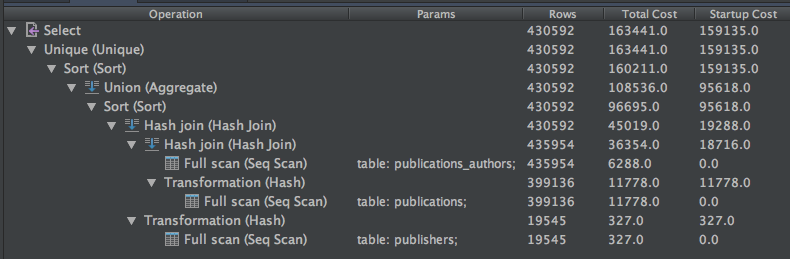
\includegraphics[scale = 0.5]{./query_analysis/query16}
    \caption{Running plan for this query (obtained with Datagrip)}
\end{figure}

\newpage

\subsection{Query 3 : Find the author who has reviewed the most titles}

\subsubsection{Initial query}
		\begin{lstlisting}[language=SQL,showspaces=false,basicstyle=\ttfamily,numberstyle=\tiny,commentstyle=\color{gray}]
SELECT a.name
FROM authors a
WHERE a.id = (
  SELECT pa.author_id
  FROM publications p
    INNER JOIN publications_authors pa ON pa.publication_id = p.id
    INNER JOIN publications_contents pc ON pc.publication_id = p.id
    INNER JOIN titles t ON t.id = pc.title_id
  WHERE t.type = 'review'
  GROUP BY pa.author_id
  ORDER BY COUNT(DISTINCT pc.title_id) DESC
  LIMIT 1
);
		\end{lstlisting}

~\\
To achieve his goal this query will use the title type \texttt{review} to filter out the titles that aren't reviews. Then it will group by \texttt{author\char`_id} to count for each author the number of distinct titles that are reviews.
~\\
		
\subsubsection{Running time \& optimization}

This query runs in approximately \textbf{1.1 second}. After the scans and joins we already spent 85\% of the time. The rest is taken by the sort for the group by clause on \texttt{pa.author\char`_id}. 


\subsubsection{Plan}
The join is first applied on \texttt{titles} and \texttt{publications\char`_contents}, then on \texttt{publications} and finally on ~\\ \texttt{publications\char`_authors}.

\begin{figure}[!htb]
	\centering
    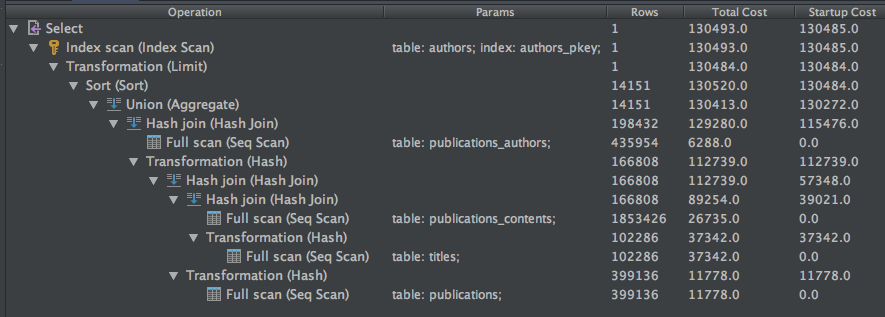
\includegraphics[scale = 0.5]{./query_analysis/query21}
    \caption{Running plan for this query (obtained with Datagrip)}
\end{figure}


\end{document}
